\chapter{Properties of Triangles}
In this chapter we will study the relations between the sides and trigonometrical ratios of the angles of a triangle. We already
know that a triangle has three sides and three angles. In a $\triangle ABC$ we will denote the angles $BAC, CBA, ACB$
by $A, B, C$ and the corresponsing sides i.e. sides opposite to them by $a, b, c$ respectively.

Thus, $BC = a, AC = b, AB = c$

We will also denote the radius of the circumcircle of the $\triangle ABC$ by $R$ and the area by $\triangle.$ We
also know some basic properties of a triangle for example, $A + B  + C = 180^\circ$ and $a + b > c, b + c > a, c + a >
b$.

\section{Sine Formula or Sine Rule or Law of Sines}
\begin{theorem}
  In $\triangle ABC, \frac{a}{\sin A} = \frac{b}{\sin B} = \frac{c}{\sin C}$
\end{theorem}

\begin{proof}
  \textbf{Case I:} When $\angle C$ is accute.
  \begin{figure}
  \begin{center}
    \begin{tikzpicture}
      \draw (-2,0) -- (2, 0) -- (0, 3) -- cycle;
      \draw [blue] (-2, 0) node[anchor=north east] {$B$};
      \draw [blue] (2, 0) node[anchor=north west] {$C$};
      \draw [blue] (0, 3) node[anchor=south] {$A$};
      \draw [dashed] (0, 3) -- (0, 0);
      \coordinate (A) at (0, 3);
      \coordinate (B) at (-2, 0);
      \coordinate (C) at (2, 0);
      \coordinate (B1) at (-2, -.5);
      \coordinate (C1) at (2, -.5);
      \draw [<->] (B1) -- (C1);
      \draw [blue] (0, 0) node[anchor=north] {$D$};
      \node [label={[black!60!green]below:$a$}] at ( $ (B1)!0.5!(C1) $ ) () {};
      \node [label={[black!60!green]above left:$c$}] at ( $ (A)!0.5!(B) $ ) () {};
      \node [label={[black!60!green]above right:$b$}] at ( $ (A)!0.5!(C) $ ) () {};
    \end{tikzpicture}
  \end{center}
  \end{figure}
  From $A$ draw $AD \perp BC$. From $\triangle ABD$,

  \noindent $\sin B = \frac{AD}{AB} = \frac{AD}{c}\Rightarrow AD = c\sin B$

  \noindent From $\triangle ACD$,

  \noindent $\sin C = \frac{AD}{AC} = \frac{AD}{b}\Rightarrow AD = b\sin C$

  \noindent Thus, $c\sin B = b\sin C$

  \textbf{Case II:} When $\angle C$ is obtuse:
  \begin{center}
    \begin{tikzpicture}
      \draw (-4,0) -- (-2, 0) -- (0, 2) -- cycle;
      \draw [blue] (-4, 0) node[anchor=north] {$B$};
      \draw [blue] (-2, 0) node[anchor=north] {$C$};
      \draw [blue] (0, 2) node[anchor=south] {$A$};
      \draw [dashed] (-2, 0) -- (0, 0);
      \draw [dashed] (0, 0) -- (0, 2);
      \draw [blue] (0, 0) node[anchor=north] {$D$};
      \draw [black!60!green] (-2, 1) node[anchor=south east] {$c$};
      \draw [black!60!green] (-3, 0) node[anchor=north] {$a$};
      \draw [black!60!green] (-1, 1) node[anchor=west] {$b$};
      \coordinate (A) at (0, 2);
      \coordinate (B) at (-4, 0);
      \coordinate (C) at (-2, 0);
      \coordinate (D) at (0, 0);
      \pic [draw, black!60!green, "$C$", angle eccentricity=1.5] {angle = A--C--B};
      \pic [draw, black!60!green, "$\pi - C$", angle eccentricity=2] {angle = D--C--A};
    \end{tikzpicture}
  \end{center}
  From $A$ draw $AD \perp BC$. From $\triangle ABD$,

  \noindent $\sin B = \frac{AD}{AB} = \frac{AD}{c}\Rightarrow AD = c\sin B$

  \noindent From $\triangle ACD$,

  \noindent $\sin(\pi - C) = \frac{AD}{AC} = \frac{AD}{b}\Rightarrow AD = b\sin C$

  \noindent Thus, $c\sin B = b\sin C$

  \textbf{Case III:} When $\angle C$ is $90^\circ$:
  \begin{center}
    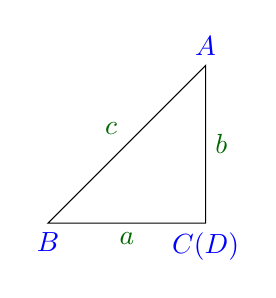
\begin{tikzpicture}
      \draw (-2,0) -- (0, 0) -- (0, 2) -- cycle;
      \draw [blue] (-2, 0) node[anchor=north] {$B$};
      \draw [blue] (0, 0) node[anchor=north] {$C(D)$};
      \draw [blue] (0, 2) node[anchor=south] {$A$};
      \draw [black!60!green] (-1, 1) node[anchor=south east] {$c$};
      \draw [black!60!green] (-1, 0) node[anchor=north] {$a$};
      \draw [black!60!green] (0, 1) node[anchor=west] {$b$};
    \end{tikzpicture}
  \end{center}
  From $A$ draw $AD \perp BC.$ From $\triangle ABD,$

  \noindent $\sin B = \frac{AD}{AB} = \frac{AD}{c}\Rightarrow AD = c\sin B$ $\Rightarrow AC = c\sin B[\because C$ and $D$ are same points $]$

  \noindent$b = c\sin B \Rightarrow b\sin90^\circ = c\sin B$ $\Rightarrow b\sin C = c\sin B$

  \noindent Thus, from all cases we have established that $\frac{b}{\sin B} = \frac{c}{\sin C}$

  \noindent Similarly by drawing perpendicular from $C$ to $AB,$ we can prove that

  \noindent $\frac{a}{\sin A} = \frac{b}{\sin B}$ and thus $\triangle ABC, \frac{a}{\sin A} = \frac{b}{\sin B} = \frac{c}{\sin C}$
\end{proof}

\begin{theorem}
  In a $\triangle ABC, \frac{a}{\sin A} = \frac{b}{\sin B} = \frac{c}{\sin C} = 2R$, where $R$ is the radius of the circumcircle of
  $\triangle ABC$.
\end{theorem}

\begin{proof}
  \textbf{Case I:} When $\angle A$ is acute.
  \begin{center}
    \begin{tikzpicture}
      \draw (0,0) circle (2cm);
      \coordinate [label={[blue]below:$O$}] (O) at (0,0);
      \draw (0.1, -0.1) -- (-0.1, 0.1);
      \coordinate [label={[blue]above:$A$}] (A) at (-.5, 1.94);
      \coordinate [label={[blue]above right:$D$}] (D) at (1.3, 1.52);
      \coordinate [label={[blue]right:$C$}] (C) at (1.3, -1.52);
      \coordinate [label={[blue]left:$B$}] (B) at (-1.3, -1.52);
      \draw (B) -- (C);
      \draw (A) -- (B);
      \draw (B) -- (D);
      \draw (C) -- (A);
      \draw (C) -- (D);
      \node[label={[black!60!green]left:$c$}] at ( $ (A)!0.5!(B) $ ) () {};
      \node[label={[black!60!green]below:$a$}] at ( $ (C)!0.5!(B) $ ) () {};
      \node[label={[black!60!green]above right:$b$}] at ( $ (C)!0.5!(A) $ ) () {};
      \node[label={[black!60!green]above left:$2R$}] at ( $ (B)!0.5!(D) $ ) () {};
      \draw pic [draw, angle radius=0.2cm] {angle=B--A--C};
      \coordinate [label={[label distance=0.3cm, black!60!green]below:$A$}] (A1) at (-.5, 1.94);
      \draw pic [draw, angle radius=0.2cm] {angle=B--D--C};
      \coordinate [label={[black!60!green]below left:$A$}] (D1) at (1.3, 1.52);
      \draw pic [draw, angle radius=0.2cm] {angle=D--C--B};
      \coordinate [label={[black!60!green]above left:$90^\circ$}] (C) at (1.3, -1.52);
    \end{tikzpicture}
  \end{center}
  From $\triangle BDC, \sin A = \frac{BC}{BD} = \frac{a}{2R} \Rightarrow \frac{a}{\sin A} = 2R$.

  \noindent\textbf{Case II:} When $\angle A$ is obtuse.
  \begin{center}
    \begin{tikzpicture}
      \draw (0,0) circle (2cm);
      \coordinate [label={[blue]below:$O$}] (O) at (0,0);
      \draw (0.1, 0.1) -- (-0.1, -0.1);
      \coordinate [label={[blue]above:$A$}] (A) at (0, 2);
      \coordinate [label={[blue]right:$D$}] (D) at (1.94, -.5);
      \coordinate [label={[blue]right:$C$}] (C) at (1.94, .5);
      \coordinate [label={[blue]left:$B$}] (B) at (-1.94, .5);
      \draw (B) -- (C);
      \draw (A) -- (B);
      \draw (B) -- (D);
      \draw (C) -- (A);
      \draw (C) -- (D);
      \node[label={[black!60!green]left:$c$}] at ( $ (A)!0.5!(B) $ ) () {};
      \node[label={[black!60!green]above:$a$}] at ( $ (C)!0.5!(B) $ ) () {};
      \node[label={[black!60!green]right:$b$}] at ( $ (C)!0.5!(A) $ ) () {};
      \node[label={[black!60!green]above:$2R$}] at ( $ (B)!0.5!(D) $ ) () {};
      \draw pic [draw, angle radius=0.2cm] {angle=B--A--C};
      \coordinate [label={[label distance=0.3cm, black!60!green]below:$A$}] (A1) at (0, 2);
      \draw pic [draw, angle radius=0.2cm] {angle=C--D--B};
      \coordinate [label={[label distance=0.3cm,black!60!green]above left:$\pi - A$}] (D1) at (1.94, -.5);
    \end{tikzpicture}
  \end{center}
  From $\triangle BDC, \sin(\pi - A) = \frac{BC}{BD} = \frac{a}{2R} \Rightarrow \frac{a}{\sin A} = 2R$.

  \noindent\textbf{Case III:} When $\angle A$ is $90^\circ$.
  \begin{center}
    \begin{tikzpicture}
      \draw (0,0) circle (2cm);
      \coordinate [label={[blue]below:$O$}] (O) at (0,0);
      \draw (0, 0.1) -- (-0, -0.1);
      \coordinate [label={[blue]above:$A$}] (A) at (0, 2);
      \coordinate [label={[blue]right:$C$}] (C) at (2, 0);
      \coordinate [label={[blue]left:$B$}] (B) at (-2, 0);
      \draw (B) -- (C);
      \draw (A) -- (B);
      \draw (C) -- (A);
      \node[label={[black!60!green]left:$c$}] at ( $ (A)!0.5!(B) $ ) () {};
      \node[label={[black!60!green]above:$a$}] at ( $ (C)!0.5!(B) $ ) () {};
      \node[label={[black!60!green]right:$b$}] at ( $ (C)!0.5!(A) $ ) () {};
      \draw pic [draw, angle radius=0.2cm] {angle=B--A--C};
      \coordinate [label={[label distance=0.3cm, black!60!green]below:$90^\circ$}] (A1) at (0, 2);
    \end{tikzpicture}
  \end{center}
  From $\triangle BDC, a = BC = 2R \Rightarrow \frac{a}{\sin A} = 2R$.

  \noindent Similarly, by joining the diameter through $A$ and $O$ and through $C$ and $O$, we can show that $\frac{b}{\sin B} =
  \frac{c}{\sin C} = 2R$.

  \noindent Hence proved.
\end{proof}

\section{Tangent Rule}
\begin{theorem}
  In any $\triangle ABC$,
  $$\tan\frac{B - C}{2} = \frac{b - c}{b + c}\cot\frac{A}{2}, \tan\frac{A - B}{2} = \frac{a - b}{a + b}\cot\frac{C}{2},
  \text{~and~}\tan\frac{C - A}{2} = \frac{c - a}{c + a}\cot\frac{B}{2}.$$
\end{theorem}

\begin{proof}
  By sine formula, $\frac{a}{\sin A} = \frac{b}{\sin B} = \frac{c}{\sin C} = K$ (say)

  $$\therefore b = K\sin B, c = k\sin C$$
  $$\therefore \frac{b - c}{b + c} = \frac{K(\sin B - \sin C)}{K(\sin B + \sin C)} = \frac{2\cos\frac{B + C}{2}\sin\frac{B -
      C}{2}}{2\sin\frac{B + C}{2}\cos\frac{B - C}{2}}$$
  $$=\cot\frac{B + C}{2}\tan\frac{B - C}{2} = \tan\frac{A}{2}\tan\frac{B - C}{2} \Rightarrow \tan\frac{B - C}{2} = \frac{b - c}{b +
    c}\cot\frac{A}{2}.$$
  Hence proved.
\end{proof}

Similarly, we can prove the two other equations.

\section{Cosine Formula or Cosine Rule}
\begin{theorem}
  In any $\triangle ABC, \cos A = \frac{b^2 + c^2 - a^2}{2bc}, \cos B = \frac{c^2 + a^2 - b^2}{2ca}, \cos C = \frac{a^2 + b^2 - c^2}{2ab}.$
\end{theorem}

\begin{proof}
  \textbf{Case I:} When $\angle C$ is acute.
  \begin{figure}[ht]
    \begin{center}
      \begin{tikzpicture}
        \draw (-2,0) -- (2, 0) -- (0, 3) -- cycle;
        \draw [blue] (-2, 0) node[anchor=north east] {$B$};
        \draw [blue] (2, 0) node[anchor=north west] {$C$};
        \draw [blue] (0, 3) node[anchor=south] {$A$};
        \draw [dashed] (0, 3) -- (0, 0);
        \coordinate (A) at (0, 3);
        \coordinate (B) at (-2, 0);
        \coordinate (C) at (2, 0);
        \coordinate (B1) at (-2, -.5);
        \coordinate (C1) at (2, -.5);
        \draw [<->] (B1) -- (C1);
        \draw [blue] (0, 0) node[anchor=north] {$D$};
        \node [label={[black!60!green]below:$a$}] at ( $ (B1)!0.5!(C1) $ ) () {};
        \node [label={[black!60!green]above left:$c$}] at ( $ (A)!0.5!(B) $ ) () {};
        \node [label={[black!60!green]above right:$b$}] at ( $ (A)!0.5!(C) $ ) () {};
      \end{tikzpicture}
    \end{center}
  \end{figure}
  $AD = b\sin C, \cos C = \frac{CD}{AC}\Rightarrow CD = b\cos C \Rightarrow BD = BC - CD = a - b\cos C$.

  \noindent\textbf{Case I:} When $\angle C$ is obtuse.
  \begin{center}
    \begin{tikzpicture}
      \draw (-4,0) -- (-2, 0) -- (0, 2) -- cycle;
      \draw [blue] (-4, 0) node[anchor=north] {$B$};
      \draw [blue] (-2, 0) node[anchor=north] {$C$};
      \draw [blue] (0, 2) node[anchor=south] {$A$};
      \draw [dashed] (-2, 0) -- (0, 0);
      \draw [dashed] (0, 0) -- (0, 2);
      \draw [blue] (0, 0) node[anchor=north] {$D$};
      \draw [black!60!green] (-2, 1) node[anchor=south east] {$c$};
      \draw [black!60!green] (-3, 0) node[anchor=north] {$a$};
      \draw [black!60!green] (-1, 1) node[anchor=west] {$b$};
      \coordinate (A) at (0, 2);
      \coordinate (B) at (-4, 0);
      \coordinate (C) at (-2, 0);
      \coordinate (D) at (0, 0);
      \pic [draw, black!60!green, "$C$", angle eccentricity=1.5] {angle = A--C--B};
      \pic [draw, black!60!green, "$\pi - C$", angle eccentricity=2] {angle = D--C--A};
    \end{tikzpicture}
  \end{center}
  $AD = b\sin(\pi - C) = b\sin C, \cos(\pi - C) = \frac{CD}{AC}\Rightarrow CD = -\cos C \Rightarrow BC = BC + CD = a - b\cos C$.

  \noindent\textbf{Case III:} When $\angle C$ is $90^\circ$.
  \begin{center}
    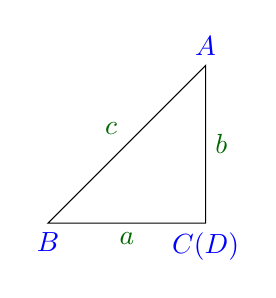
\begin{tikzpicture}
      \draw (-2,0) -- (0, 0) -- (0, 2) -- cycle;
      \draw [blue] (-2, 0) node[anchor=north] {$B$};
      \draw [blue] (0, 0) node[anchor=north] {$C(D)$};
      \draw [blue] (0, 2) node[anchor=south] {$A$};
      \draw [black!60!green] (-1, 1) node[anchor=south east] {$c$};
      \draw [black!60!green] (-1, 0) node[anchor=north] {$a$};
      \draw [black!60!green] (0, 1) node[anchor=west] {$b$};
    \end{tikzpicture}
  \end{center}
  Here, $C$ and $D$ are same points. $AD = AC = b = b\sin C, CD = 0 = b\cos C [\because \cos C = \cos90^\circ = 0]$

  \noindent $BD = BC - CD = a - b\cos C$, thus, in all cases $AD = b\sin C$ and $BD = a - b\cos C$

  \noindent Now, $AB^2 = AD^2 + BD^2 \Rightarrow c^2 = b^2\sin^2C + (a - b\cos C)^2 \Rightarrow \cos C = \frac{a^2 + b^2 - c^2}{2ab}$.

  Hence proved.
\end{proof}
Similarly, we can prove it for $\angle A$ and $\angle B$.

\section{Projection Formulae}
\begin{theorem}
  In any $\triangle ABC, c = a\cos B + b\cos A, b = c\cos A + a\cos C, a = b\cos C + c\cos B$.
\end{theorem}

\begin{proof}
  \noindent \textbf{Case I:} When $\angle C$ is acute.
  \begin{figure}[ht]
    \begin{center}
      \begin{tikzpicture}
        \draw (-2,0) -- (2, 0) -- (0, 3) -- cycle;
        \draw [blue] (-2, 0) node[anchor=north east] {$B$};
        \draw [blue] (2, 0) node[anchor=north west] {$C$};
        \draw [blue] (0, 3) node[anchor=south] {$A$};
        \draw [dashed] (0, 3) -- (0, 0);
        \coordinate (A) at (0, 3);
        \coordinate (B) at (-2, 0);
        \coordinate (C) at (2, 0);
        \coordinate (B1) at (-2, -.5);
        \coordinate (C1) at (2, -.5);
        \draw [<->] (B1) -- (C1);
        \draw [blue] (0, 0) node[anchor=north] {$D$};
        \node [label={[black!60!green]below:$a$}] at ( $ (B1)!0.5!(C1) $ ) () {};
        \node [label={[black!60!green]above left:$c$}] at ( $ (A)!0.5!(B) $ ) () {};
        \node [label={[black!60!green]above right:$b$}] at ( $ (A)!0.5!(C) $ ) () {};
      \end{tikzpicture}
    \end{center}
  \end{figure}
  $BC = a = BD + CD = c\cos B + b\cos C$.

  \noindent \textbf{Case II:} When $\angle C$ is obtuse.
  \begin{center}
    \begin{tikzpicture}
      \draw (-4,0) -- (-2, 0) -- (0, 2) -- cycle;
      \draw [blue] (-4, 0) node[anchor=north] {$B$};
      \draw [blue] (-2, 0) node[anchor=north] {$C$};
      \draw [blue] (0, 2) node[anchor=south] {$A$};
      \draw [dashed] (-2, 0) -- (0, 0);
      \draw [dashed] (0, 0) -- (0, 2);
      \draw [blue] (0, 0) node[anchor=north] {$D$};
      \draw [black!60!green] (-2, 1) node[anchor=south east] {$c$};
      \draw [black!60!green] (-3, 0) node[anchor=north] {$a$};
      \draw [black!60!green] (-1, 1) node[anchor=west] {$b$};
      \coordinate (A) at (0, 2);
      \coordinate (B) at (-4, 0);
      \coordinate (C) at (-2, 0);
      \coordinate (D) at (0, 0);
      \pic [draw, black!60!green, "$C$", angle eccentricity=1.5] {angle = A--C--B};
      \pic [draw, black!60!green, "$\pi - C$", angle eccentricity=2] {angle = D--C--A};
    \end{tikzpicture}
  \end{center}
  $BC = a = BD - CD = c\cos B - b\cos(\pi - C) = c\cos B + b\cos C$
  \noindent \textbf{Case III:} When $\angle C$ is $90^\circ$.
  \begin{center}
    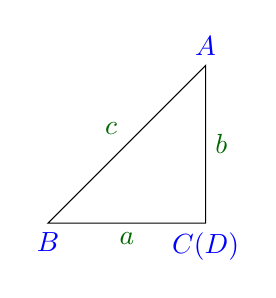
\begin{tikzpicture}
      \draw (-2,0) -- (0, 0) -- (0, 2) -- cycle;
      \draw [blue] (-2, 0) node[anchor=north] {$B$};
      \draw [blue] (0, 0) node[anchor=north] {$C(D)$};
      \draw [blue] (0, 2) node[anchor=south] {$A$};
      \draw [black!60!green] (-1, 1) node[anchor=south east] {$c$};
      \draw [black!60!green] (-1, 0) node[anchor=north] {$a$};
      \draw [black!60!green] (0, 1) node[anchor=west] {$b$};
    \end{tikzpicture}
  \end{center}
  $BD = a = BC + CD = c\cos B + b\cos C[\because C=90^\circ \therefore \cos C = 0]$

  \noindent Thus, in all cases $a = b\cos C + c\cos B$. Similarly, we can prove for other sides.
\end{proof}

\section{Sub-Angle Rules}
\begin{theorem}
  In any $\triangle ABC, \sin\frac{A}{2}= \sqrt{\frac{(s - b)(s - c)}{bc}}, \cos\frac{A}{2} = \sqrt{\frac{s(s - a)}{bc}},
  \tan\frac{A}{2} = \sqrt{\frac{(s - b)(s - c)}{s(s - a)}}$, where $2s = a + b + c$.
\end{theorem}

\begin{proof}
  $$2\sin^2\frac{A}{2} = 1 - \cos A = 1 - \frac{b^2 + c^2 - a^2}{2bc} = \frac{a^2 - (b - c)^2}{2bc} = \frac{(a + b - c)(a + c -
    b)}{2bc}$$
  $$= \frac{(2s - 2c)(2s - 2b)}{2bc} \Rightarrow \sin^2\frac{A}{2} = \frac{(s - b)(s - c)}{bc}$$
  $$\Rightarrow \sin\frac{A}{2} = \pm\sqrt{\frac{(s - b)(s - c)}{bc}}$$
  But $\frac{A}{2}$ is an acute angle so $\sin\frac{A}{2}> 0$ $$\therefore \sin\frac{A}{2} = \sqrt{\frac{(s - b)(s - c)}{bc}}$$

  $$2\cos^2\frac{A}{2} = 1 + \cos A = 1 + \frac{b^2 + c^2 - a^2}{2bc} = \frac{(b + c)^2 - a^2}{2bc} = \frac{(a + b + c)(b + c -
    a)}{2bc}$$
  $$= \frac{(2s)(2s - 2a)}{2bc} \Rightarrow \cos^2\frac{A}{2} = \frac{s(s - a)}{bc}$$
  $$\Rightarrow \cos\frac{A}{2} = \pm\sqrt{\frac{s(s - a)}{bc}}$$
  But $\frac{A}{2}$ is an acute angle is $\cos\frac{A}{2} > 0$ $$\therefore \cos\frac{A}{2} = \sqrt{\frac{s(s - a)}{bc}}$$

  \noindent From the two equation which we have found it follows that $\tan\frac{A}{2} = \sqrt{\frac{(s - b)(s - c)}{s(s -
      a)}}$. Similarly, we can prove the relations for other angles.
\end{proof}

\section{Sines of Angles in Terms of Sides}
\begin{theorem}
  In any $\triangle ABC$, $\sin A = \frac{2}{bc}\sqrt{s(s - a)(s - b(s - c)}, \sin B = \frac{2}{ca}\sqrt{s(s - a)(s - b(s - c)},$
  $\sin C = \frac{2}{ab}\sqrt{s(s - a)(s - b(s - c)}$.
\end{theorem}

\begin{proof}
  $$\sin A = 2\sin\frac{A}{2}\cos\frac{A}{2} = 2\sqrt{\frac{(s - b)(s - c)}{bc}}\sqrt{\frac{s(s - a)}{bc}} = \frac{2}{bc}\sqrt{s(s
    - a)(s - b(s - c)}$$

  \noindent Similarly, we can prove it for other angles.
\end{proof}

\section{Area of a Triangle}
\begin{theorem}
  If $\Delta$ denotes the area of $\triangle ABC,$ then
  $$\Delta = \frac{1}{2}ab\sin C = \frac{1}{2}bc\sin A = \frac{1}{2}ca\sin B.$$
\end{theorem}

\begin{proof}
  \noindent \textbf{Case I:} When $\angle C$ is acute.
    \begin{center}
      \begin{tikzpicture}
        \draw (-2,0) -- (2, 0) -- (0, 3) -- cycle;
        \draw [blue] (-2, 0) node[anchor=north east] {$B$};
        \draw [blue] (2, 0) node[anchor=north west] {$C$};
        \draw [blue] (0, 3) node[anchor=south] {$A$};
        \draw [dashed] (0, 3) -- (0, 0);
        \coordinate (A) at (0, 3);
        \coordinate (B) at (-2, 0);
        \coordinate (C) at (2, 0);
        \coordinate (B1) at (-2, -.5);
        \coordinate (C1) at (2, -.5);
        \draw [<->] (B1) -- (C1);
        \draw [blue] (0, 0) node[anchor=north] {$D$};
        \node [label={[black!60!green]below:$a$}] at ( $ (B1)!0.5!(C1) $ ) () {};
        \node [label={[black!60!green]above left:$c$}] at ( $ (A)!0.5!(B) $ ) () {};
        \node [label={[black!60!green]above right:$b$}] at ( $ (A)!0.5!(C) $ ) () {};
      \end{tikzpicture}
    \end{center}

  $\sin C = \frac{AD}{AC}\Rightarrow AD = b\sin C \therefore \Delta = \frac{1}{2}BC\times AD = \frac{1}{2}ab\sin C$.

  \noindent \textbf{Case II:} When $\angle C$ is obtuse.
  \begin{center}
    \begin{tikzpicture}
      \draw (-4,0) -- (-2, 0) -- (0, 2) -- cycle;
      \draw [blue] (-4, 0) node[anchor=north] {$B$};
      \draw [blue] (-2, 0) node[anchor=north] {$C$};
      \draw [blue] (0, 2) node[anchor=south] {$A$};
      \draw [dashed] (-2, 0) -- (0, 0);
      \draw [dashed] (0, 0) -- (0, 2);
      \draw [blue] (0, 0) node[anchor=north] {$D$};
      \draw [black!60!green] (-2, 1) node[anchor=south east] {$c$};
      \draw [black!60!green] (-3, 0) node[anchor=north] {$a$};
      \draw [black!60!green] (-1, 1) node[anchor=west] {$b$};
      \coordinate (A) at (0, 2);
      \coordinate (B) at (-4, 0);
      \coordinate (C) at (-2, 0);
      \coordinate (D) at (0, 0);
      \pic [draw, black!60!green, "$C$", angle eccentricity=1.5] {angle = A--C--B};
      \pic [draw, black!60!green, "$\pi - C$", angle eccentricity=2] {angle = D--C--A};
    \end{tikzpicture}
  \end{center}
  $\sin(\pi - C) = \frac{AD}{AC} \Rightarrow AD = b\sin C \therefore \Delta = \frac{1}{2}BC\times AD = \frac{1}{2}ab\sin C$.

  \noindent \textbf{Case III:} When $\angle C$ is $90^\circ$.
  \begin{center}
    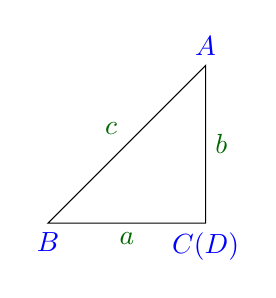
\begin{tikzpicture}
      \draw (-2,0) -- (0, 0) -- (0, 2) -- cycle;
      \draw [blue] (-2, 0) node[anchor=north] {$B$};
      \draw [blue] (0, 0) node[anchor=north] {$C(D)$};
      \draw [blue] (0, 2) node[anchor=south] {$A$};
      \draw [black!60!green] (-1, 1) node[anchor=south east] {$c$};
      \draw [black!60!green] (-1, 0) node[anchor=north] {$a$};
      \draw [black!60!green] (0, 1) node[anchor=west] {$b$};
    \end{tikzpicture}
  \end{center}
  $\Delta = \frac{1}{2}BC\times AD = \frac{1}{2}ab\sin C[\because C=90^\circ \therefore \sin C = 1]$.

  \noindent Thus in all cases $\Delta = \frac{1}{2}ab\sin C$. Similarly, we can prove two other formulae.
\end{proof}

\section{Area in Terms of Sides}
\begin{theorem}
  If $\Delta$ be the area of any $\triangle ABC$, when $\Delta = \sqrt{s(s - a)(s - b)(s - c)}$.
\end{theorem}

\begin{proof}
  $$\Delta = \frac{1}{2}ab\sin C = \frac{1}{2}ab.2\sin\frac{C}{2}\cos\frac{C}{2} = ab\sqrt{\frac{(s - a)(s -
      b)}{ab}}.\sqrt{\frac{s(s - c)}{ab}}$$
  $$= \sqrt{s(s - a)(s - b)(s - c)}.$$

  \noindent Hence proved.
\end{proof}

\subsection{Area in Terms of Radius of Circumcircle}
$$\Delta = \frac{1}{2}ab\sin C = \frac{1}{2}ab.\frac{c}{2R} = \frac{abc}{4R}.$$

\section{Tangent and Cotangent of Sub-angles of a Triangle}
\begin{theorem}
  In any $\triangle ABC$,
  $$\tan\frac{A}{2} = \frac{(s - b)(s - c)}{\Delta}, \tan\frac{B}{2} = \frac{(s - a)(s - c)}{\Delta}, \tan\frac{C}{2} = \frac{(s -
    a)(s - c)}{\Delta},$$
  $$\cos\frac{A}{2} = \frac{s(s - a)}{\Delta}, \cot\frac{B}{2} = \frac{s(s - b)}{\Delta}, \cot\frac{C}{2} = \frac{s(s -
    c)}{\Delta}.$$
\end{theorem}

\begin{proof}
  $$\tan\frac{A}{2} = \sqrt{\frac{(s - b)(s - c)}{s(s - a)}} = \sqrt{\frac{(s - b)^2(s - c)^2}{s(s - a)(s - b)(s - c)}}$$
  $$= \frac{(s - b)(s - c)}{\Delta}.$$

  \noindent Similarly, we can prove for other angles and cotangents.
\end{proof}

\section{Dividing a Side in a Ratio}
\begin{theorem}
  If $D$ be a point on the side $BC$ of a $\triangle ABC$ such that $BD:dC = m:n$ and $\angle ADC = \theta, \angle BAD = \alpha$
  and $\angle DAC = \beta$, then
  $$(m + n)\cot\theta = m\cot\alpha - n\cot\beta,$$
  $$(m + n)\cot\theta = n\cot B - m\cot C.$$
  \begin{center}
    \begin{tikzpicture}
      \coordinate [label={[blue]above:$A$}] (A) at (0, 2);
      \coordinate [label={[blue]right:$C$}] (C) at (2, 0);
      \coordinate [label={[blue]left:$B$}] (B) at (-2, 0);
      \coordinate [label={[blue]below:$D$}] (D) at (-0.2, 0);
      \draw (B) -- (C);
      \draw (A) -- (B);
      \draw (C) -- (A);
      \draw (D) -- (A);
      \node[label={[black!60!green]left:$c$}] at ( $ (A)!0.5!(B) $ ) () {};
      \node[label={[black!60!green]below, xshift=0.5cm, yshift=0.1cm:$a$}] at ( $ (C)!0.5!(B) $ ) () {};
      \node[label={[black!60!green]right:$b$}] at ( $ (C)!0.5!(A) $ ) () {};
      \draw pic [draw, angle radius=0.2cm] {angle=B--A--C};
      \draw pic [draw, angle radius=0.2cm] {angle=C--B--A};
      \draw pic [draw, angle radius=0.2cm] {angle=A--C--B};
      \draw pic [draw, angle radius=0.3cm] {angle=A--D--B};
      \draw pic [draw, angle radius=0.3cm] {angle=C--D--B};
      \coordinate [label={[label distance=0.3cm, black!60!green]below left, xshift=0.2cm:$\alpha$}] (A1) at (0, 2);
      \coordinate [label={[label distance=0.3cm, black!60!green]below right, xshift=-0.3cm:$\beta$}] (A1) at (0, 2);
      \coordinate [label={[label distance=0.3cm, black!60!green]above right:$\theta$}] (D1) at (-0.2, 0);
      \coordinate [label={[label distance=0.3cm, black!60!green]above left, xshift=0.2cm:$\pi-\theta$}] (D1) at (-0.2, 0);
    \end{tikzpicture}
  \end{center}
\end{theorem}

\begin{proof}
  $$\angle ADB = \pi - \theta, \angle ABD = \pi - (\alpha + \pi - \theta) = \theta - \alpha, \angle ACD = \pi - (\theta + \beta).$$
  From $\triangle ABC, \frac{BD}{\sin\alpha} = \frac{AD}{\sin(\theta - \alpha)}$. Form $\triangle ADC, \frac{DC}{\sin\beta} =
  \frac{AB}{\sin[\pi - (\theta + \beta)]}$.

  \noindent Dividing, we get $$\frac{BD\sin\beta}{DC\sin\alpha} = \frac{\sin(\theta + \beta)}{\sin(\theta - \alpha)}$$
  $$\Rightarrow \frac{m\sin\beta}{n\sin\alpha} = \frac{\sin\theta\cos\beta + \cos\theta\cos\beta}{\sin\theta\cos\alpha -
    \cos\theta\sin\alpha}$$
  $$\Rightarrow m\sin\theta\sin\beta\cos\alpha - m\cos\theta\sin\alpha\sin\beta = n\sin\alpha\sin\theta\cos\beta +
  n\sin\alpha\cos\theta\sin\beta$$
  Dividing boths ides by $\sin\alpha\sin\beta\sin\theta$, we get
  $$m\cot\alpha - m\cot\theta = n\cot\beta + n\cot\theta$$
  $$\Rightarrow (m + n)\cot\theta = n\cot\beta + n\cot\theta.$$

  \noindent Thus, first part is proved and now we will prove the second part.
  $$\angle BAD = 180^\circ - (180^\circ - \theta + B) = \theta - B, \angle DAC = 180^\circ - (\theta + C)$$
  From $\triangle BAD, \frac{BD}{\sin(\theta - B)} = \frac{AD}{\sin B}$. From $\triangle ADC, \frac{DC}{\sin[180^\circ - (\theta +
      C)]} = \frac{AD}{\sin C}$
  $$\Rightarrow \frac{DC}{\sin(\theta + c)} = \frac{AD}{\sin C}$$
  Dividing, we get
  $$\frac{BD}{DC}.\frac{\sin(\theta + C)}{\sin(\theta - B)} = \frac{\sin C}{\sin B}$$
  $$\Rightarrow \frac{m}{n}.\frac{\sin\theta\cos C + \cos\theta\sin C}{\sin\theta\cos B - \cos\theta\sin B} = 1$$
  Proceeding like previous proof, we have
  $$(m + n)\cot\theta = n\cot B - m\cot C.$$
  Hence proved.
\end{proof}

\section{Results Related with Circumcircle}
A circle passing through the vertices of a triangle is called a circumcircle. Its radius is called the circumradius.
\begin{theorem}
  Let $O$ be the center of the circumscribing circle of $\triangle ABC$. Then, $R = \frac{abc}{4\Delta}$.
  \begin{center}
    \begin{tikzpicture}
      \draw (0, 0) circle(2);
      \coordinate [label={[blue]above:$A$}] (A) at (0, 2);
      \coordinate [label={[blue]right:$C$}] (C) at (1.732, -1);
      \coordinate [label={[blue]left:$B$}] (B) at (-1.732, -1);
      \coordinate [label={[blue]below:$O$}] (O) at (0, 0);
      \draw (B) -- (C);
      \draw (A) -- (B);
      \draw (C) -- (A);
      \draw (O) -- (A);
      \draw (O) -- (B);
      \draw (O) -- (C);
      \coordinate [label={[label distance=0.2cm, black!60!green] above right:$R$}] (A2) at (0, 0);
      \node[label={[black!60!green]:$=$}] at ( $ (A)!0.5!(O) $ ) (A1) {};
      \node[label={[black!60!green, rotate=60, yshift=-.2cm, xshift=-0.1cm]:$=$}] at ( $ (C)!0.5!(O) $ ) (C1) {};
      \node[label={[black!60!green, rotate=120, yshift=-.2cm, xshift=-0.1cm]:$=$}] at ( $ (B)!0.5!(O) $ ) (B1) {};
    \end{tikzpicture}
  \end{center}
\end{theorem}

\begin{proof}
  By sine rule, $$\frac{a}{\sin A} = 2R \Rightarrow R = \frac{a}{2\sin A}$$
  $$\because \Delta = \frac{1}{2}bc\sin A \therefore \sin A = \frac{2\Delta}{bc}$$
  $$\Rightarrow R = \frac{a}{\frac{2.2\Delta}{bc}} = \frac{abc}{4\Delta}.$$
  Hence proved.
\end{proof}

\section{Results Related with Incircle}
The circle touching all the three sides of a triangle internally is called the inscribed circle or in-circle. Its radius is called
in-radius and denoted by $r$. In the figure $I$ is the incenter of the $\triangle ABC$.

Clearly, it is the point of intersection of internal bisector of angles of the $\triangle ABC$.

\begin{theorem}
  In $\triangle ABC, r = \frac{\Delta}{s}$.
  \begin{center}
    \begin{tikzpicture}
      \draw (0, 0) circle(1);
      \coordinate [label={[blue]above:$A$}] (A) at (0, 2);
      \coordinate [label={[blue]right:$C$}] (C) at (1.732, -1);
      \coordinate [label={[blue]left:$B$}] (B) at (-1.732, -1);
      \coordinate [label={[blue]above:$I$}] (I) at (0, 0);
      \coordinate [label={[blue]below:$D$}] (D) at (0, -1);
      \coordinate [label={[blue]above right:$E$}] (E) at (.866, 0.5);
      \coordinate [label={[blue]above left:$F$}] (F) at (-.866, 0.5);
      \draw (B) -- (C);
      \draw (A) -- (B);
      \draw (C) -- (A);
      \draw (I) -- (D);
      \draw (I) -- (E);
      \draw (I) -- (F);
      \coordinate [label={[label distance=0.2cm, black!60!green] below right:$R$}] (A2) at (0, 0);
      \node[label={[black!60!green, yshift=-0.3cm]:$=$}] at (0, -.5 ) (A1) {};
      \node[label={[black!60!green, rotate=120, yshift=-.2cm, xshift=-0.1cm]:$=$}] at ( $ (E)!0.5!(I) $ ) (C1) {};
      \node[label={[black!60!green, rotate=240, yshift=-.2cm, xshift=0.1cm]:$=$}] at ( $ (F)!0.5!(I) $ ) (B1) {};
    \end{tikzpicture}
  \end{center}
\end{theorem}

\begin{proof}
  $$\text{Area of~}\triangle ABC = \triangle IBC + \triangle ICA + \triangle IAB$$
  $$\Rightarrow \Delta = \frac{1}{2}ar + \frac{1}{2}br + \frac{1}{2}cr \Rightarrow r = \frac{\Delta}{s}$$
  Hence proved.
\end{proof}

\subsection{Other Forms}
\begin{enumerate}
\item $r = 4R\sin\frac{A}{2}\sin\frac{B}{2}\sin\frac{C}{2}$

  R.H.S. $= 4.\frac{abc}{4\Delta}.\sqrt{\frac{(s - b)(s - c)}{bc}}.\sqrt{\frac{(s - a)(s - c)}{ca}}.\sqrt{\frac{(s - a)(s - b)}{ab}}$

  $= \frac{abc}{\Delta}.\frac{(s - a)(s - b)(s - c)}{abc}.\frac{s}{s} = \frac{abc}{\Delta}.\frac{\Delta}{s} = \frac{\Delta}{s} = r$.
\item $r = (s - a)\tan\frac{A}{2} = (s - b)\tan\frac{B}{2} = (s - c)\tan\frac{C}{2}$

  $r = \frac{\Delta}{s} = \frac{\Delta}{s}.\frac{s - a}{s - a} = (s - a)\tan\frac{A}{2}$.

  Similarly, we can prove for other angles.
\end{enumerate}

\section{Results Related with Escribed Circles}
Let $ABC$ be a triangle. Let the bisectors of exterior angles $B$ and $C$ meet at $I_1$. Let $I_1D\perp BC$. If we take $I_1$ as
the center aand draw a circle it will touch all the three sides(two extended) of the triangle. We can draw three such circles, one
opposite to each side. We denote these radii by $r_1, r_2$ and $r_3$ for angle s$A, B$ and $C$ respectively.
\begin{theorem}
  In such a $\triangle ABC, r_1 = \frac{\Delta}{s - a}, r_2 = \frac{\Delta}{s - b}, r_3 = \frac{\Delta}{s - c}$.
\begin{center}
  \includegraphics[scale=0.5]{16_1_10}
  \label{fig:esc}
\end{center}
\end{theorem}

\begin{proof}
  $$\Delta ABC = \Delta I_1AB + \Delta I_1AC - \Delta I_1BC$$
  $$=\frac{1}{2}cr_1 + \frac{1}{2}br_1 - \frac{1}{2}ar_1 = \frac{1}{2}(2s - 2a)r_1 = (s - a)r_1$$
  $$\Rightarrow r_1 = \frac{\Delta}{s - a}.$$
  Similarly, it can be proven for $r_2$ and $r_3$.
\end{proof}

\subsection{Other Forms}
\begin{enumerate}
\item $r_1 = s\tan\frac{A}{2} = 4R\sin\frac{A}{2}\cos\frac{B}{2}\cos\frac{C}{2}$
\item $r_2 = s\tan\frac{B}{2} = 4R\cos\frac{A}{2}\sin\frac{B}{2}\cos\frac{C}{2}$
\item $r_3 = s\tan\frac{C}{2} = 4R\cos\frac{A}{2}\cos\frac{B}{2}\sin\frac{C}{2}$
\end{enumerate}

\section{Distannces of Centers from Vertices}
We have already shown that for circumcenter distance is equal to circum-radius i.e. $R$.

Referring to the image of incircle, $IF = r, \angle FAI = \frac{A}{2}$. From right-angle $\triangle FIA, \sin\frac{A}{2} =
\frac{r}{AI}\Rightarrow AI = r{\rm cosec}\frac{A}{2}$.

Similarly, $BI = r{\rm cosec}\frac{B}{2}$ and $CI = r{\rm cosec}\frac{C}{2}$.

\subsection{Orthocenter}
Orthocenter is the point of intersection of perpendiculars from a vertex to opposite side.
\begin{center}
  \begin{tikzpicture}
    \coordinate [label={[blue]above:$A$}] (A) at (0, 2);
    \coordinate [label={[blue]right:$C$}] (C) at (1.732, -1);
    \coordinate [label={[blue]left:$B$}] (B) at (-.732, -1);
    \draw (B) -- (C);
    \draw (A) -- (B);
    \draw [name path=AC] (C) -- (A);
    \draw ($(A)!(B)!(C)$) -- (B);
    \draw ($(B)!(A)!(C)$) -- (A);
    \draw ($(B)!(C)!(A)$) -- (C);
    \node [label={[blue]$E$}] () at ($(A)!(B)!(C)$) {};
    \node [label={[blue]below:$D$}] () at ($(B)!(A)!(C)$) {};
    \node [label={[blue]$F$}] () at ($(B)!(C)!(A)$) {};
    \MarkRightAngle {A}{$(B)!(A)!(C)$}{B};
    \MarkRightAngle {B}{$(A)!(B)!(C)$}{C};
    \MarkRightAngle {C}{$(B)!(C)!(A)$}{B};
  \end{tikzpicture}
\end{center}
Let the orthocenter be $H$ which is intersection of perpendiculars from any vertex to opposite side. From right-angle $\triangle
AEB, \cos A = \frac{AE}{AB}\Rightarrow AE = c\cos A$

From right-angle $\triangle ACD, \angle DAC = 90^\circ - C$. From right-angle $\triangle AEH, \cos(90^\circ - C) = \frac{AE}{AH}$

$\Rightarrow AH = \frac{c\cos A}{\sin C} = 2R\cos A$. Similarly, $BH = 2R\cos B$ and $CH = 2R\cos C$.

\subsection{Centroid}
\begin{center}
  \begin{tikzpicture}
    \coordinate [label={[blue]above:$A$}] (A) at (0, 2);
    \coordinate [label={[blue]right:$C$}] (C) at (2, 0);
    \coordinate [label={[blue]left:$B$}] (B) at (-2, 0);
    \coordinate [label={[blue]below:$D$}] (D) at (0, 0);
    \draw (B) -- (C);
    \draw (A) -- (B);
    \draw [name path=AC] (C) -- (A);
    \draw (D) -- (A);
    \node [label={[black!60!green]below, xshift=0.3cm:$a$}] at ( $ (B)!0.5!(C) $ ) () {};
    \node [label={[black!60!green]above left:$c$}] at ( $ (A)!0.5!(B) $ ) () {};
    \node [label={[black!60!green]above right:$b$}] at ( $ (A)!0.5!(C) $ ) () {};
    \node [label={[blue]:$-$}] at (0, .3) () {};
    \node [label={[blue]left:$G$}] at (0, .66) () {};
  \end{tikzpicture}
\end{center}
Let $G$ be the centroid. Since, it is the point of intersection of medians, it will lie on median $AD$.

From geometry, $AB^2 + AC^2 = 2BD^2 + 2AD^2 \Rightarrow c^2 + b^2 = 2.\frac{a^2}{4} + 2AD^2$

$\Rightarrow 2AD^2 = \frac{2b^2 + 2c^2 - a^2}{2}$

$\because AG:GD = 2:1$ [property of centeroid that it divides median in the ratio $2:1$]

$AG = \frac{2}{3}AD = \frac{1}{2}\sqrt{2b^2 + 2c^2 - a^2}$. Similarly, $BG = \frac{1}{3}\sqrt{2a^2 + 2c^2 - b^2}$ and $CG =
\frac{1}{3}\sqrt{2a^2 + 2b^2 - c^2}$.

\subsubsection{Angles Made by Medians with Sides}
If $\angle BAD = \beta$ and $\angle CAD = \gamma$, then we have $\frac{\sin\gamma}{\sin C} = \frac{DC}{AD} \Rightarrow \sin\gamma =
\frac{DC.\sin C}{AD}$

$= \frac{a\sin C}{\sqrt{2b^2 + 2c^2 - a^2}}$. Similarly, $\sin\beta = \frac{a\sin B}{\sqrt{2b^2 + 2c^2 - a^2}}$.

If $\angle ADC$ be $theta$ then we have $\sin\theta = \frac{2b\sin C}{2b^2 + 2c^2 - a^2}$.

\section{Escribed Triangles}
Refer to Figure {\ref{fig:esc}}, in which $I$ is the incenter and $I_1, I_2$ and $I_3$ are the centers of the excircles opposite to
vertices $A, B$ and $C$ respectively. We know that $IC$ will bisect the $\angle ACB, I_1C$ will bisect the external angles at $C$
and $I_1B$ will bisect the angle at $B$ produces by extending the sides i.e. $\angle BCM$ as shown in the figure.

$\therefore \angle ICI_1 = \angle ICM + \angle ICM = \frac{1}{2}\angle ACB + \frac{1}{2}\angle BCM = 90^\circ$.

Similarly, $\angle ICI_1$ and $\angle ICI_3$ will be right angles.

Hence $I_1CI_2$ is perpendicular to $IC$. Similarly, $I_2AI_3$ is perpendicular to $IA$, and $I_1BI_3$ is perpendicular to $IB$.

We also see that $IA$ and $I_1A$ bot bisect $\angle A$ so $AII_1$ is a straight line. Similarly $I_2IB$ and $I_3IC$ are straight
lines.
The $\triangle I_1I_2I_3$ is called the \textit{excentric} triangle of $\triangle ABC$.

\section{Distance between Orthocenter and Circumcenter}
Let $O$ be the circumcenter. $OF\perp AAB$ and $H$ be orthocenter. Then $\angle OAF = 90^\circ - \angle AOF = 90^\circ - C$.

Let $BL\perp AC$ so it will pass through $H$. $\angle HAL = 90^\circ - C, \angle OAH = A - \angle OAF - \angle HAL = A - (180^circ
- 2C) = C - B$

Also, $OA = R$ and $HA = 2R\cos A. OH^2 = OA^2 + HA^2 - 2OA.HA.\cos OAH = R^2 + 4R^2\cos^2A - 4R^2\cos^2A - 4R^2\cos A\cos(C - B)$

$= R^2 + 4R^2\cos A[\cos A - \cos(C - B)] = R^2 - 8R^2\cos A\cos B\cos C$

$\Rightarrow OH = R\sqrt{1 - 8\cos A\cos B\cos C}$.

\section{Distance between Incenter and Circumcenter}
Let $O$ be the orthocenter and $OF\perp AB$. Let $I$ be the incenter and $IC\perp AB$.

$\angle OAF = 90^\circ - C \therefore \angle OAI = \angle IAF - \angle OAF = \frac{A}{2} - 90^\circ + C = \frac{C - B}{2}$.

Also, $AI = \frac{IE}{\sin\frac{A}{2}} = \frac{r}{\sin\frac{A}{2}} = 4R\sin\frac{B}{2}\sin\frac{C}{2}$.

$\therefore OI^2 = OA^2 + AI^2 - 2.OA.AI.\cos OAI$

$ = R^2 + 16R^2\sin^2\frac{B}{2}\sin^2\frac{C}{2} - 8R^2\sin\frac{B}{2}\sin\frac{C}{2}\cos\frac{C - B}{2}$

$OI = R\sqrt{1 - 8\sin\frac{A}{2}\sin\frac{B}{2}\sin\frac{C}{2}} = \sqrt{R^2 - 2Rr}$.

\section{Area of a Cyclic Quadrilateral}
\begin{theorem}
  \begin{center}
    \begin{tikzpicture}
      \draw (1, 1) circle(1.414);
      \coordinate [label={[blue]left:$A$}] (A) at (0, 2);
      \coordinate [label={[blue]right:$C$}] (C) at (2, 0);
      \coordinate [label={[blue]right:$B$}] (B) at (2, 2);
      \coordinate [label={[blue]left:$D$}] (D) at (0, 0);
      \draw (B) -- (C);
      \draw (A) -- (B);
      \draw (C) -- (D);
      \draw (D) -- (A);
      \draw (C) -- (A);
      \node [label={[black!60!green]right :$b$}] at ( $ (B)!0.5!(C) $ ) () {};
      \node [label={[black!60!green]above:$a$}] at ( $ (A)!0.5!(B) $ ) () {};
      \node [label={[black!60!green]below:$c$}] at ( $ (C)!0.5!(D) $ ) () {};
      \node [label={[black!60!green]left:$d$}] at ( $ (D)!0.5!(A) $ ) () {};
    \end{tikzpicture}
  \end{center}

  If $a, b, c, d$ be the sides and $s$ be the subperimeter of a cyclic quadrilateral, then its area is $\sqrt{(s - a)(s - b)(s -
    c)(s - d)}$.
\end{theorem}

\begin{proof}
  Let $ABCD$ be a cyclic quadrilateral having sides $AB = a, BC = b, CD = c$ and $AD = d$. Since opposing angles of a quadrilateral
  are complementary, therefore $B + D = A + C = \pi$.

  Applying cosine law in $\triangle ABC, \cos B = \frac{a^2 + b^2 - AC^2}{2ab}\Rightarrow AC^2 = a^2 + b^2 - 2ab\cos B$.

  Similarly in $\triangle ACD, AC^2 = c^2 + d^2 + 2cd \cos B$. Thus, $\cos B = \frac{a^2 + b^2 - c^2 - d^2}{2(ab + cd)}$.

  Area of quadrilaterl $ABCD = \Delta ABC + \Delta ACD = \frac{1}{2}ad\sin B + \frac{1}{2}cd \sin B$

  Solving last two equations, we get area of quadrilateral $= \sqrt{(s - a)(s - b)(s - c)(s - d)}$.
\end{proof}

\section{Problems}
\begin{enumerate}
\item The sides of a triangle are $8$ cm, $10$ cm and $12$ cm. Prove that the greatest angle is double the smallest
   angle.

\item In a $\triangle ABC,$ if $\frac{b + c}{11} = \frac{c + a}{12} = \frac{a + b}{13},$ prove that $\frac{\cos
   A}{7} = \frac{\cos B}{19} = \frac{\cos C}{25}$

\item If $\triangle = a^2 - (b - c)^2,$ where $\triangle$ is the area of the $\triangle ABC,$ then prove that
   $\tan A = \frac{8}{15}$

\item In a triangle $ABC,$ the angles $A, B, C$ are in A.P. Prove that $2\cos\frac{A - C}{2} = \frac{a +
   c}{\sqrt{a^2 - ac + c^2}}$

\item If $p_1, p_2, p_3$ be the altitudes of a triangle $ABC$ from the vertices $A, B, C$ respectively and
   $\Delta$ be the area of the triangle, prove that $\frac{1}{p_1} + \frac{1}{p_2} - \frac{1}{p_3} =
   \frac{2ab\cos^2\frac{C}{2}}{\Delta(a + b + c)}$

\item In any $\triangle ABC,$ if $\tan\theta = \frac{2\sqrt{ab}}{a - b}\sin\frac{C}{2},$ prove that $c = (a -
   b)\sec\theta$

\item In a $\triangle ABC, a=6, b = 3$ and $\cos(A - B) = \frac{4}{5},$ then find its area.

\item In a $\triangle ABC, \angle C=60^\circ$ and $\angle A=75^\circ.$ If $D$ is a point on $AC$ such that
   area of $\triangle BAD$ is $\sqrt{3}$ times the area of the $\triangle BCD,$ find $\angle ABD$

\item If the sides of a triangle are $3, 5$ and $7,$ prove that the triangle is obtuse angled triangle and find the obtuse
   angle.

\item In a triangle $ABC,$ if $\angle A = 45^\circ, \angle B = 75^\circ,$ prove that $a + c\sqrt{2} = 2b$

\item In a triangle $ABC, \angle C = 90^\circ, a = 3, b =4$ and $D$ is a point on $AB,$ so that $\angle
    BCD=30^\circ,$ find the length of $CD.$

\item The sides of a triangle are $4cm, 5cm$ and $6cm.$ Show that the smallest angle is half of the greatest angle.

\item In an isosceles triangle with base $a,$ the vertical angle is $10$ times any of the base angles. Find the length of
    equal sides of the triangle.

\item The angles of a triangle are in the ratio of $2:3:7,$ then prove that the sides are in the ratio of
    $\sqrt{2}:2:(\sqrt{3} + 1)$

\item In a triangle $ABC,$ if $\frac{\sin A}{7} = \frac{\sin B}{6} = \frac{\sin C}{5},$ show that $\cos A:\cos
    B:\cos C = 7:19:25$

\item In any triangle $ABC$ if $\tan\frac{A}{2} = \frac{5}{6}, \tan\frac{B}{2} = \frac{20}{37},$ find
    $\tan\frac{C}{2}$ and prove that in this triangle $a + c = 2b.$

\item In a triangle $ABC$ if $\angle C=60^\circ,$ prove that $\frac{1}{a + c} + \frac{1}{b + c} = \frac{3}{a + b +
    c}$

\item If $\alpha, \beta, \gamma$ be the lengths of the altitudes of a triangle $ABC,$ prove that
    $\frac{1}{\alpha^2} + \frac{1}{\beta^2} + \frac{1}{\gamma^2} = \frac{\cot A + \cot B + \cot C}{\Delta},$ where
    $\Delta$ is the area of the triangle.

\item In a triangle $ABC,$ if $\frac{a}{b} = 2 + \sqrt{3}$ and $\angle C= 60^\circ,$ show that $\angle A =
    105^\circ$ and $\angle B=15^\circ.$

\item If two sides of a triangle and the included angle are given by $a = (1 + \sqrt{3}), b = 2$ and $C=60^\circ,$ find
    the other two angles and the third side.

\item The sides of a triangle are $x, y$ and $\sqrt{x^2 + xy + y^2}.$ prove that the greatest angle is $120^\circ.$

\item The sides of a triangle are $2x + 3, x^2 + 3x + 3$ and $x^2 + 2x,$ prove that greatest amgle is $120^\circ.$

\item In a triangle $ABC,$ if $3a = b + c,$ prove that $\cot\frac{B}{2}\cot\frac{C}{2} = 2$

\item In a triangle $ABC,$ prove that $a\sin\left(\frac{A}{2} + B\right) = (b + c)\sin\frac{A}{2}$

\item In a triangle $ABC,$ prove that $\frac{\cot\frac{A}{2} + \cot\frac{B}{2} + \cot\frac{C}{2}}{\cot A + \cot B + \cot
    C} = \frac{(a + b + c)^2}{a^2 + b^2 + c^2}$

\item In a triangle $ABC,$ prove that $\frac{b^2 - c^2}{a^2}\sin2A + \frac{c^2 - a^2}{b^2}\sin2B + \frac{a^2 -
    b^2}{c^2}\sin2C = 0$

\item In a trianlge $ABC,$ prove that $a^3\cos(B - C) + b^3\cos(C - A) + c^3\cos(A - B) = 3abc$

\item In a triangle $ABC,$ prove that $\frac{\cos^2\frac{B - C}{2}}{(b + c)^2} + \frac{\sin^2\frac{B - C}{2}}{(b - c)^2}
    = \frac{1}{a^2}$

\item In a triangle $ABC,$ prove that $\frac{a}{\cos B\cos C} + \frac{b}{\cos C\cos A} + \frac{c}{\cos A\cos B} = 2a\tan
    B\tan C\sec A$

\item In a triangle $ABC,$ prove that $(b - c)\cos\frac{A}{2} = a\sin\frac{B - C}{2}$

\item In a triangle $ABC,$ prove that $\tan\left(\frac{A}{2} + B\right) = \frac{c + b}{c - b}\tan \frac{A}{2}$

\item In a triangle $ABC,$ prove that $\tan\frac{A - B}{2} = \frac{a - b}{a + b}\cot\frac{C}{2}$

\item In a triangle $ABC,$ prove that $(b + c)\cos A + (c + a)\cos B + (a + b)\cos C = a + b + c$

\item In a triangle $ABC,$ prove that $\frac{\cos^2B - \cos^2C}{b + c} + \frac{\cos^2C - \cos^2A}{c + a} +
    \frac{\cos^2A - \cos^2B}{a + b} = 0$

\item In a triangle $ABC,$ prove that $a^3\sin(B - C) + b^3\sin(C - A) + c^3\sin(A - B) = 0$

\item In a triangle $ABC,$ prove that $(b + c - a)\tan\frac{A}{2} = (c + a - b)\tan\frac{B}{2} = (a + b -
    c)\tan\frac{C}{2}$

\item In a triangle $ABC,$ prove that $1 - \tan\frac{A}{2}\tan\frac{B}{2} = \frac{2c}{a + b + c}$

\item In a triangle $ABC,$ prove that $\frac{\cos2A}{a^2} - \frac{\cos2B}{b^2} = \frac{1}{a^2} - \frac{1}{b^2}$

\item In a triangle $ABC,$ prove that $a^2(\cos^2B - \cos^2C) + b^2(\cos^2C - \cos^2A) + c^2(\cos^2A - \cos^2B) = 0$

\item In a triangle $ABC,$ prove that $\frac{a^2\sin(B - C)}{\sin B + \sin C} + \frac{b^2\sin(C - A)}{\sin C + \sin A} +
    \frac{c^2\sin(A - B)}{\sin A + \sin B} = 0$

\item In a triangle $ABC,$ prove that $\frac{\cos A}{a} + \frac{\cos B}{b} + \frac{\cos C}{c} = \frac{a^2 + b^2 +
    c^2}{2abc}$

\item In a triangle $ABC,$ prove that $\frac{\cos A}{a} + \frac{a}{bc} = \frac{\cos B}{b} + \frac{b}{ca} = \frac{\cos
    C}{c} + \frac{c}{ab}$

\item In a triangle $ABC,$ prove that $(b^2 - c^2)\cot A + (c^2 - a^2)\cot B + (a^2 - b^2)\cot C = 0$

\item In a triangle $ABC,$ prove that $(b - c)\cot\frac{A}{2} + (c - a)\cot\frac{B}{2} + (a - b)\cot\frac{C}{2} = 0$

\item In a triangle $ABC,$ prove that $(a - b)^2\cos^2\frac{C}{2} + (a + b)^2\sin^2\frac{C}{2} = c^2$

\item In a triangle $ABC,$ prove that $\frac{a- b}{a + b} = \cot\frac{A + B}{2}\tan\frac{A - B}{2}$

\item In a triangle $ABC, D$ is the middle point of $BC.$ If $AD$ is perpendicular to $AC,$ prove that
    $\cos A\cos C = \frac{2(c^2 - a^2)}{3ac}$

\item If $D$ be the middle point of the side $BC$ of the triangle $ABC$ where area is $\Delta$ and
    $\angle ADB=\theta,$ prove that $\frac{AC^2 - AB^2}{4\Delta} = \cot\theta$

\item $ABCD$ is a trapezium such that $AB$ and $DC$ are parallel and $BC$ is perpendicular to the. If
    $\angle ADB = \theta, BC = p, CD=q,$ show that $AB = \frac{(p^2 + q^2)\sin\theta}{p\cos\theta + q\sin\theta}$

\item Let $O$ be a point inside a triangle $ABC$ such that $\angle OAB = \angle OBC = \angle OCA = \theta,$ show
    that $\cot \theta = \cot A + \cot B + \cot C.$

\item The median $AD$ of a triangle $ABC$ is perpendicular to $AB.$ Prove that $\tan A + 2\tan B = 0.$

\item In a triangle $ABC,$ if $\cot A+ \cot B + \cot C = \sqrt{3}$

\item In a triangle $ABC,$ if $(a^2 + b^2)\sin(A - B) = (a^2 - b^2)\sin(A + B)$

\item In a triangle $ABC,$ if $\theta$ be any angle, show that $b\cos\theta = c\cos(A - \theta) + a\cos(C +
    \theta)$

\item In a triangle $ABC, AD$ is the median. If $\angle BAD = \theta,$ prove that $\cos\theta = 2\cot A + \cot B$

\item The bisector of angle $A$ of a triangle $ABC$ meets $BC$ in $D,$ show that $AD = \frac{2bc}{b +
    c}\cos \frac{A}{2}$

\item Let $A$ and $B$ be two points on one bank of a straight river and $C$ and $D$ be two points on the
    other bank, the direction from $A$ to $B$ along the river being the same as from $C$ to $D.$ If
    $AB = a, \angle CAD = \alpha, \angle DAB = \beta, \angle CBA=\gamma,$ prove that $CD =
    \frac{a\sin\alpha\sin\gamma}{\sin\beta \sin(\alpha + \beta + \gamma)}$

\item In a triangle $ABC,$ if $2\cos A = \frac{\sin B}{\sin C},$ prove that the triangle is isosceles.

\item If the cosines of two angles of a triangle are inversely proportional to the opposite sides, show that the triangle is either
    isosceles or right angled.

\item In a triangle $ABC,$ if $a\tan A + b\tan B = (a + b)\tan\frac{A + B}{2},$ prove that the triangle is isosceles.

\item In a triangle $ABC,$ if $\frac{\tan A - \tan B}{\tan A + \tan B} = \frac{c - b}{c},$ prove that $A =
    60^\circ$

\item In a triangle $ABC,$ if $c^4 - 2(a^2 + b^2)c^2 + a^4 + a^2b^2 + b^4 = 0,$ prove that $C=60^\circ$ or
    $120^\circ$

\item In a triangle $ABC,$ if $\frac{\cos A + 2\cos C}{\cos A + 2\cos B} = \frac{\sin B}{\sin C},$ prove that the
    triangle is either isosceles or right angled.

\item If $A, B, C$ are angles of a $\triangle ABC$ and if $\tan\frac{A}{2}, \tan\frac{B}{2}, \tan\frac{C}{2}$ are
    in A.P., prove that $\cos A, \cos B, \cos C$ are in A.P.

\item In a triangle $ABC,$ if $a\cos^2\frac{C}{2} + c\cos^2\frac{A}{2} = \frac{3b}{2},$ show that $\cot\frac{A}{2},
    \cot\frac{B}{2}, \cot\frac{C}{2}$ are in A.P.

\item If $a^2, b^2, c^2$ are in A.P., then prove that $\cot A, \cot B, \cot C$ are in A.P.

\item The angles $A, B$ and $C$ of a triangle $ABC$ are in A.P. If $2b^2 = 3c^2,$ determine the angle $A.$

\item If in a triangle $ABC, \tan\frac{A}{2}, \tan\frac{B}{2}, \tan\frac{C}{2}$ are in H.P., then show that the sides $a,
    b, c$ are in A.P.

\item In a triangle $ABC,$ if $\frac{\sin A}{\sin C} = \frac{\sin(A - B)}{\sin(B - C)},$ prove that $a^2, b^2, c^2$
    are in A.P.

\item In a triangle $ABC, \sin A, \sin B, \sin C$ are in A.P. show that $3\tan\frac{A}{2}\tan\frac{C}{2} = 1.$

\item In a triangle $ABC,$ if $a^2, b^2, c^2$ are in A.P., show that $\tan A, \tan B, \tan C$ are in H.P.

\item In a triangle $ABC,$ if $a^2, b^2, c^2$ are in A.P., show that $\cot A, \cot B, \cot C$ are in A.P.

\item If the angles $A, B, C$ of a triangle $ABC$ be in A.P. and $b:c = \sqrt{3}:\sqrt{2},$ find the angle
    $A.$

\item The sides of a triangle are in A.P. and the greatest angle exceeds the least angle by $90^\circ.$ Prove that the sides
    are in the ratio $\sqrt{7} + 1: \sqrt{7}: \sqrt{7} - 1.$

\item If the sides $a, b, c$ of a triangle are in A.P. and if $a$ is the least side, prove that $\cos A =
    \frac{4c - 3b}{2c}$

\item The two adjacent sides of a cyclic quadrilateral are $2$ and $5$ nad the angle between them is $60^\circ.$ If
    the third side is $3,$ find the fourth side.

\item Find the angle $A$ of triangle $ABC,$ in which $(a + b + c)(b + c - a) = 3bc$

\item If in a triangle $ABC, \angle A = \frac{\pi}{3}$ and $AD$ is a median, then prove that $4AD^2 = b^2 + bc +
    c^2$

\item Prove that the median $AD$ and $BE$ of a $\Delta ABC$ intersect at right angle if $a^2 + b^2 = 5c^2$

\item If in a triangle $ABC, \frac{\tan A}{1} = \frac{\tan B}{2} = \frac{\tan C}{3},$ then prove that $6\sqrt{2}a =
    3\sqrt{5}b = 2\sqrt{10}c$

\item The sides of a triangle are $x^2 + x + 1, 2x + 1$ and $x^2 - 1,$ prove that the greatest anngle is $120^\circ.$

\item The sides of a triangle are three consecutive natural numbers and its largest angle is twice the smallest one. Determine the
    sides of the triangle.

\item For a triangle $ABC$ having area $12$ sq. cm. and base is $6$ cm. The difference of base angles is
    $60^\circ.$ Show that angle $A$ opposite to the base is given by $8\sin A - 6\cos A = 3.$

\item In any triangle $ABC,$ if $\cos\theta = \frac{a}{b + c}, \cos\phi = \frac{b}{a + c}, \cos\psi = \frac{c}{a +
    b}$ where $\theta, \phi$ and $\psi$ lie between $0$ and $\pi,$ prove that
    $\tan^2\frac{\theta}{2} + \tan^2\frac{\phi}{2} + \tan^2\frac{\psi}{2} = 1.$

\item In a triangle $ABC,$ if $\cos A\cos B + \sin A\sin B\sin C = 1,$ show that the sides are in the proportion
    $1:1:\sqrt{2}.$

\item The product of the sines of the angles of a triangle is $p$ and the product of their cosines is $q.$ Show that the
    tangents of the angles are the roots of the equation $qx^3 - px^2 + (1 + q)x - p = 0$

\item In a $\triangle ANC,$ if $\sin^3\theta = \sin(A - \theta)\sin(B - \theta)\sin(C - \theta),$ prove that $\cot\theta
    = \cot A + \cot B + \cot C.$

\item In a triangle of base $a,$ the ratio of the other two sides is $r(< 1),$ show that the altitude of the triangle is
    less than or equal to $\frac{ar}{1 - r^2}$

\item Given the base $a$ of a triangle, the opposite angle $A,$ and the product $k^2$ of the other two sides. Solve
    the triangle and show that there is such triangle if $a < 2k\sin\frac{A}{2}, k$ being positive.

\item A ring $10$ cm in diameter, is suspended from a point $12$ cm above its center by $6$ equal strings, attached
    at equal intervals. Find the cosine of the angle between consecutive strings.

\item If $2b = 3a$ and $\tan^2\frac{A}{2} = \frac{3}{5},$ prove that there are two values of third side, one of which is
    double the other.

\item The angles of a triangle are in the ratio $1:2:7,$ prove that the ratio of the greater side to the least side is
    $\sqrt{5} + 1:\sqrt{5} - 1.$

\item If $f, g, h$ are internal bisectors of the angles of a triangle $ABC,$ show that
    $\frac{1}{f}\cos\frac{A}{2} + \frac{1}{g}\cos\frac{B}{2} + \frac{1}{h}\cos\frac{C}{2} = \frac{1}{a} + \frac{1}{b} +
    \frac{1}{c}.$

\item If in a triangle $ABC, BC = 5, CA = 4, AB = 3$ and $D$ and $E$ are points on $BC$ scuh that $BD =
    DE = EC.$ If $\angle CAB=\theta,$ then prove that $\tan\theta = \frac{3}{8}.$

\item In a triangle $ABC,$ median $AD$ and $CE$ are drawn. If $AD = 5, \angle DAC = \frac{\pi}{8}$ and
    $\angle ACE = \frac{\pi}{4},$ find the area of the triangle $ABC.$

\item The sides of a triangle are $7, 4\sqrt{3}$ and $\sqrt{13}$ cm. Then prove that the smallest angle is
    $30^\circ.$

\item In an isosceles, right angled triangle a straight line is drawn from the middle point of one of the equal sides to the opposite
    angle. Show that it divides the angle in two parts whose cotangents are $2$ and $3.$

\item The sides of a triangle are such that $\frac{a}{1 + m^2n^2} = \frac{b}{m^2 + n^2} = \frac{c}{(1- m^2)(1 + n^2)},$ prove
    that $A = 2\tan^{-1}\frac{m}{n}, B = 2\tan^{-1}mn$ and $\Delta = \frac{mnbc}{m^2 + n^2}.$

\item The sides $a, b, c$ if a triangle $ABC$ are the roots of the equation $x^3 - px^2 + qx - r = 0,$ prove that
    its area is $\frac{1}{4}\sqrt{p(4pq - p^3 - 8r)}$

\item Two sides of a triangle are of lengths $\sqrt{6}$ cm and $4$ cm and the angle opposite to the smaller side is
     $30^\circ.$ How many such triangles are possible? Fine the length of their third side and area.

\item The base of a triangle is divided into three equal parts. If $t_1, t_2, t_3$ be the tangents of the angles subtended by
     these parts at the opposite vertex, prove that $\left(\frac{1}{t_1} + \frac{1}{t_2}\right)\left(\frac{1}{t_2} +
     \frac{1}{t_3}\right) = 4\left(1 + \frac{1}{t_2^2}\right)$

\item The three medians of a triangle $ABC$ make angles $\alpha, \beta, \gamma$ with each other, prove that
     $\cot\alpha + \cot\beta + \cot\gamma + \cot A + \cot B + \cot C = 0.$

\item Perpendiculars are drawn from the angles $A, B, C$ of an acute angled triangle on the opposite sides and produced to
     meet the circumscribing circle. If these produced parts be $\alpha, \beta, \gamma$ respectively, show that
     $\frac{a}{\alpha} + \frac{b}{\beta} + \frac{c}{\gamma} = 2(\tan A + \tan B + \tan C)$

\item In a triangle $ABC,$ the vertices $A, B, C$ are at distance $p, q, r$ from the orthocenter
     respectively. Show that $aqr + brp + cpq = abc$

\item The area of a circular plot of land in the form of a unit circle is to be divided into two equal parts by the arc of a circle
     whose center is on the circumference of the plot. Show that the radius of the circular arc is given by $\cos\theta$
     where $\theta$ is given by $\frac{\pi}{2} = \sin2\theta - 2\theta\cos2\theta$

\item $BC$ is a side of a square, on the perpendicular bisector of $BC,$ two points $P, Q$ are taken, equidistant
     from the center of square. $BP$ and $CQ$ are joined and cut in $A.$ Prove that in the trangle $ABC,$
     $\tan A(\tan B - \tan C)^2 + 8 = 0$

\item If the bisector of the angle $C$ of a triangle $ABC$ cuts $AB$ in $D$ and the circum-circle in
     $E,$ prove that $CE:DE = (a + b)^2:c^2.$

\item The internal bisectors of the angles of a triangle $ABC$ meet the sides at $D, E$ and $F.$ Show that the
     area of the triangle $DEF$ is equal to $\frac{2\Delta abc}{(b + c)(c + a)(a + b)}$

\item In a triangle $ABC,$ the measures of the angles $A, B$ and $C$ are $3\alpha, 3\beta$ and
     $3\gamma$ respectively. $P, Q$ and $R$ are the points within the triangle such that $\angle BAR =
     \angle RAQ = \angle QAC = \alpha,$ $\angle CBP = \angle PBR = \angle RBA = \beta$ and $\angle ACQ = \angle QCP =
     \angle PCB = \gamma.$ Show that $AR = 8R\sin\beta\sin\gamma\cos(30^\circ - \gamma)$

\item A circle touches the $x$ axis at $O$ (origin) and intersects the $y$ axis above origin at $B. A$ is a
     point on that part of cirlce which lies to the  right of $OB,$ and the tangents at $A$ and $B$ meet at
     $T.$ If $\angle AOB = \theta,$ find the angles which the directed line $OA, AT$ and $OB$ makes with
     $OX.$ If lengths of these lines are $c, t$ and $d$ respectively, show that $c\sin\theta - t(1 +
     \cos2\theta) = 0$ and $c\cos\theta + t\sin2\theta = d.$

\item If in a triangle $ABC,$ the median $AD$ and the perpendicular $AE$ from the vertex $A$ to the side
     $BC$ divides the angle $A$ into three equal parts, show that $\cos\frac{A}{3}.\sin^2\frac{A}{3} =
     \frac{3a^2}{32bc}$

\item In a triangle $ABC,$ if $\cos A + \cos B + \cos C = \frac{3}{2},$ prove that the triangle is equilateral.

\item Prove that a triangle $ABC$ is equilateral if and only if $\tan A + \tan B + \tan C = 3\sqrt{3}.$

\item In a triangle $ABC,$ prove that $(a + b + c)\tan\frac{C}{2} = a\cot\frac{A}{2} + b\cot\frac{B}{2} -
     c\cot\frac{C}{2}$

\item In a triangle $ABC,$ prove that $\sin^4A + \sin^4B + \sin^4C = \frac{3}{2} + 2\cos A\cos B\cos C + \frac{1}{2}\cos
     2A + \cos 2B + \cos 2C$

\item In a triangle $ABC$ prove that $\cos^4A + \cos^4B + \cos^4C = \frac{1}{2} - 2\cos A\cos B\cos C + \frac{1}{2}\cos
     2A\cos 2B\cos 2C$

\item In a triangle $ABC,$ prove that $\cot B + \frac{\cos C}{\cos A\sin B} = \cot C + \frac{\cos B}{\cos A\sin C}$

\item In a triangle $ABC,$ prove that $\frac{a\sin(B - C)}{b^2 - c^2} = \frac{b\sin(C - A)}{c^2 - a^2} = \frac{c\sin(A -
     B)}{a^2 - b^2}$

\item In a triangle $ABC,$ prove that $\sin\frac{B - C}{2} = \frac{b - c}{a}\cos \frac{A}{2}$

\item In a triangle $ABC,$ prove that $\sin^3A\cos(B - C) + \sin^3B\cos(C - A) + \sin^3C\cos(A - B) = 3\sin A\sin B\sin
     C$

\item In a triangle $ABC,$ prove that $\sin^3A + \sin^3B + \sin^3C = 3\cos\frac{A}{2}\cos\frac{B}{2}\cos\frac{C}{2} +
     \cos\frac{3A}{2}\cos\frac{3B}{2}\cos\frac{3C}{2}$

\item In a triangle $ABC,$ prove that $\sin3A\sin^3(B - C) + \sin3B\sin^3(C - A) + \sin3C\sin^3(A - B) = 0$

\item In a triangle $ABC,$ prove that $\sin3A\cos^3(B - C) + \sin3B\cos^3(C - A) + \sin3C\cos^3(A - B) = \sin 3A\sin
     3B\sin 3C$

\item In a triangle $ABC,$ prove that $\left(\cot\frac{A}{2} + \cot\frac{B}{2}\right)\left(a\sin^2\frac{B}{2} +
     b\sin^2\frac{A}{2}\right) = c\cot\frac{C}{2}$

\item The sides of a triangle $ABC$ are in A.P. If the angles $A$ and $C$ are the greatest and the smallest angles
     respectively, prove that $4(1 - \cos A)(1 - \cos C) = \cos A + \cos C$

\item In a triangle $ABC,$ if $a, b, c$ are in H.P., prove that $\sin^2\frac{A}{2}, \sin^2\frac{B}{2},
     \sin^2\frac{C}{2}$ are also in H.P.

\item If the sides $a, b, c$ of a triangle $ABC$ be in A.P., prove that $\cos A\cot\frac{A}{2}, \cos
     B\cot\frac{B}{2}, \cos C\cot\frac{C}{2}$ are in A.P.

\item The sides of a triangle are in A.P. and its area is $\frac{3}{5}$ th of an equilateral triangle of the same
     perimieter. Prove that the sides are in the ratio $3:5:7.$

\item If the tangents of the angles of a triangle are in A.P., prove that the squares of the sides are in the proportion
     $x^2(x^2 + 9): (3 + x^2)^2:9(1 + x^2),$ where $x$ is the least or the greatest tangent.

\item If the sides of a triangle are in A.P. and if its greatest angle exceeds the least angle by $\alpha,$ show that the
     sides are in the ratio $1 - x:1:1 + x$ where $x = \sqrt{\frac{1 - \cos\alpha}{7 - \cos\alpha}}$

\item If the sides of triangle $ABC$ are in G.P. with common ratio $r(r>1),$ show that $r<\frac{1}{2}(\sqrt{5} +
     1)$ and $A<B<\frac{\pi}{3}<C$

\item If $p$ and $q$ be the perpendiculars from the vertices $A$ and $B$ on any line passing through the
     vertex $C$ of the triangle $ABC$ but not passing through the interior of the angle $ABC,$ prove that
     $a^2p^2 + b^2q^2 - 2abpq\cos C = a^2b^2\sin^2C$

\item $ABC$ is a triangle, $O$ is a point inside the triangle such that $\angle OAB = \angle OBC = \angle OCA =
     \theta,$ then show that ${\rm cosec}^2\theta = {\rm cosec}^2A + {\rm cosec}^2B + {\rm cosec}^2C$

\item If $x, y, z$ be the lengths of perpendiculars from the circumcenter on the sides $BC, CA, AB$ of a triangle
     $ABC,$ prove that $\frac{a}{x} + \frac{b}{y} + \frac{c}{z} = \frac{abc}{4xyz}$

\item In any triangle $ABC$ if $D$ is any point on the base $BC$ such that $BD:DC = m:n$ and if
     $AD=x,$ prove that $(m + n)^2x^2 = (m + n)(mb^2 + nc^2) - mna^2$

\item In a triangle $ABC,$ if $\sin A + \sin B + \sin C = \frac{3\sqrt{3}}{2},$ prove that the triangle is equilateral.

\item In a triangle $ABC,$ if $\sin\frac{A}{2}\sin\frac{B}{2}\sin\frac{C}{2} = \frac{1}{8},$ prove that the triangle is
     equilateral.

\item In a triangle $ABC,$ if $\cos A + 2\cos B + \cos C = 2,$ prove that the sides of the triangle are in A.P.

\item The sides $a, b, c$ of a triangle $ABC$ of a triangle are in A.P., then find the value of $\tan\frac{A}{2} +
   \tan\frac{C}{2}$ in terms of $\cot\frac{B}{2}.$

\item In a triangle $ABC,$ if $\frac{a - b}{b - c}= \frac{s - a}{s - c},$ prove that $r_1, r_2, r_3$ are in A.P.

\item If the sides $a, b, c$ of a triangle $ABC$ are in G.P., then prove that $x, y, z$ are also in G.P., where
   $x = (b^2 - c^2)\frac{\tan B + \tan C}{\tan B - \tan C}, y = (c^2 - a^2)\frac{\tan C + \tan A}{\tan C - \tan A}, z =
   (a^2 - b^2)\frac{\tan A + \tan B}{\tan A - \tan B}$

\item The ex-radii $r_1, r_2, r_3$ of a triangle $ABC$ are in H.P. Show that its sides $a, b, c$ are in A.P.

\item In usual notation, $r_1 = r_2 + r_3 + r,$ prove that the triangle is right-angled.

\item If $A, B, C$ are the angles of a triangle, prove that $\cos A + \cos B + \cos C = 1 + \frac{r}{R}$

\item Show that the radii of the three escribed circles of a triangle are the roots of the equation $x^3 - x^2(4R + r) + xs^2 -
   rs^2 = 0$

\item The radii $r_1, r_2, r_3$ of escribed circle of a triangle $ABC$ are in H.P. If its area if $24$ sq. cm. and
   its perimeter is $24$ cm., find the length of its sides.

\item In a triangle $ABC, 8R^2 = a^2 + b^2 + c^2,$ prove that the triangle is right-angled.

\item The radius of the circle passing through the center of the inscribed circle and through the point of the base $BC$ is
   $\frac{a}{2}\sec\frac{A}{2}$

\item Three circles touch each other externally. The tangents at their point of connect meet at a point whose distance from the point
   of contact is $4.$ Find the ratio of the product of radii to the sum of of radii of all the circles.

\item In a triangle $ABC,$ if $O$ be the circumcenter and $H,$ the orthocenter, show that $OH = R\sqrt{1 -
   8\cos A\cos B\cos C}$

\item Let $ABC$ be a triangle having $O$ and $I$ as its circumcenter an in-center respectively. If $R$ and
   $r$ be the circumradius and in-radius respectively, then prove that $(IO)^2 = R^2 - 2Rr.$ Further show that the
   triangle $BIO$ is a right angled triangle if and only if $b$ is the arithmetic means of $a$ and $c.$

\item In any triangle $ABC,$ prove that $\cot\frac{A}{2} + \cot\frac{B}{2} + \cot\frac{C}{2} =
   \cot\frac{A}{2}\cot\frac{B}{2}\cot\frac{C}{2}$

\item Let $ABC$ be a triangle with in-center $I$ and in-radius $r.$ Let $D, E$ and $F$ be the feet of
   perpendiculars from $I$ to the sides $BC, CA$ and $AB$ respectively. If $r_1, r_2$ and $r_3$ are
   the radii of circles inscribed in the quadrilaterals $AFIE, BDIF$ and $CEID$ respectively, prove that
   $\frac{r_1}{r - r_1} + \frac{r_2}{r - r_2} + \frac{r_3}{r - r_3} = \frac{r_1r_2r_3}{(r - r_1)(r - r_2)(r - r_3)}$

\item Show that the line joining the orthocenter to the circumference of a triangle $ABC$ is inclined to $BC$ at an angle
   $\tan^{-1}\left(\frac{3 - \tan B\tan C}{\tan B - \tan C}\right)$

\item If a circle be drawn touching the inscribed and circumscribed circle of a triangle and $BC$ externally, prove that its
   radius is $\frac{\Delta}{a}\tan^2\frac{A}{2}.$

\item The bisectors of the angles of a triangle $ABC$ meet its circumcenter in the position $D, E, F.$ Show that the area
   of the triangle $DEF$ is to that of $ABC$ is $R:2r.$

\item If the bisectors of the angles of a triangle $ABC$ meet the opposite sides in $A', B', C',$ prove that the ratio of
   the areas of the triangles $A'B'C'$ and $ABC$ is $2\sin\frac{A}{2}\sin\frac{B}{2}\sin\frac{C}{2}:\cos\frac{A -
   B}{2}\cos\frac{B - C}{2}\cos\frac{C - A}{2}.$

\item If $a, b, c$ are the sides of a triangle $\lambda a, \lambda b, \lambda c$ the sides of a similar triangle inscribed
   in the former and $\theta$ the angle between the sides of $a$ and $\lambda a,$ prove that
   $2\lambda\cos\theta = 1.$

\item If $r$ be the radius of in-circle and $r_1, r_2, r_3$ be the ex-radii of a triangle $ABC,$ prove that
   $r_1 + r_2 + r_3 - r = 4R$

\item If $r$ be the radius of in-circle and $r_1, r_2, r_3$ be the ex-radii of a triangle $ABC,$ prove that
   $\frac{1}{r_1} + \frac{1}{r_2} + \frac{1}{r_3} = \frac{1}{r}$

\item If $r$ be the radius of in-circle and $r_1, r_2, r_3$ be the ex-radii of a triangle $ABC,$ prove that
   $\frac{1}{r_1^2} + \frac{1}{r_2^2} + \frac{1}{r_3^2} + \frac{1}{r^2} = \frac{a^2 + b^2 + c^2}{\Delta^2}$ where
   $\Delta$ denotes the area of the triangle $ABC.$

\item If $r$ is the radius of in-circle of a triangle $ABC,$ prove that $r = (s - a)\tan\frac{A}{2} = (s -
   b)\tan\frac{B}{2} = (s - c)\tan\frac{C}{2}.$

\item If $A, A_1, A_2$ and $A_3$ be respectively the areas of the inscribed and escribed circles of a triangle, prove that
   $\frac{1}{\sqrt{A}} = \frac{1}{\sqrt{A_1}} + \frac{1}{\sqrt{A_2}} + \frac{1}{\sqrt{A_3}}$

\item In a triangle $ABC,$ prove that $\frac{r_1}{bc} + \frac{r_2}{ca} + \frac{r_3}{ab} = \frac{1}{r} - \frac{1}{2R}.$

\item $ABC$ is an isosceles triangle inscribed in a circle of radius $r.$ If $AB = AC$ and $h$ is the altitude
   from $A$ to $BC$ then the triangle $ABC$ has perimeter $P = 2(\sqrt{2rh - h^2} + \sqrt{2rh}).$ Find its
   area.

\item If $p_1, p_2, p_3$ are the altitudes of the triangle $ABC$ from the vertices $A, B, C$ respectively, prove
   that $\frac{\cos A}{p_1} + \frac{\cos B}{p_2} + \frac{\cos C}{p_3} = \frac{1}{R}.$

\item Three circles whose radii are $a, b, c$ touch one another externally and the tangents at their point of contact meet in a
   point. Prove that the distance of this point from either of their points of contact is $\sqrt{\frac{abc}{a + b + c}}$

\item In a triangle $ABC,$ prove that $r_1r_2r_3 = r^3\cot^2\frac{A}{2}\cot^2\frac{B}{2}\cot^2\frac{C}{2}.$

\item In a triangle $ABC,$ prove that $a(rr_1 + r2r_3) = b(rr_2 + r_3r_1) = c(rr_3 + r_1r_2) = abc.$

\item In a triangle $ABC,$ prove that $(r_1 + r_2)\tan\frac{C}{2} = (r_3 - r)\cot\frac{C}{2} = c.$

\item In a triangle $ABC,$ prove that $4R\sin A\sin B\sin C = a\cos A + b\cos B + c\cos C.$

\item In a triangle $ABC,$ prove that $(r_1 - r)(r_2 - r)(r_3 - r) = 4Rr^2$

\item In a triangle $ABC,$ prove that $r^2 + r_1^2 + r_2^2 + r_3^2 = 16R^2 - a^2 - b^2 - c^2$

\item In a triangle $ABC,$ prove that $IA. IB. IC = abc\tan\frac{A}{2}\tan\frac{B}{2}\tan\frac{C}{2}$

\item In a triangle $ABC,$ prove that $AI_1 = r_1{\rm cosec}\frac{A}{2}$

\item In a triangle $ABC,$ prove that $II_1 = a\sec\frac{A}{2}$

\item In a triangle $ABC,$ prove that $I_2I_3 = a{\rm cosec}\frac{A}{2}$

\item In a triangle $ABC,$ if $I$ is the in-center and $I_1, I_2$ and $I_3$ are the centers of the escribed
   circles, then prove that $II_1.II_2.II_3 = 16R^2r$

\item In a triangle $ABC,$ if $I$ is the in-center and $I_1, I_2$ and $I_3$ are the centers of the escribed
   circles, then prove that $II_1^2.I_2I_3^2 = II_2^2 + I_3I_1^2 = II_3^2 + I_1I_2^2 = 16R^2$

\item In a triangle $ABC,$ if $O$ is the circumcenter and $I,$ the in-center then prove that $OI^2 = R^2(3 -
   2\cos A - 2\cos B - 2\cos C).$

\item In a triangle $ABC,$ if $H$ is the orthocenter and $I$ the in-center then prove that $IH^2 = 2r^2 -
   4R^2\cos A\cos B\cos C.$

\item In a triangle $ABC,$ if $O$ is the circumcenter, $G,$ the cetroid and $H,$ the orthocenter then prove
   that $OG^2 = R^2 - \frac{1}{9}(a^2 + b^2 + c^2).$

\item Given an isosceles triangle with lateral side of length $b,$ base angle $\alpha < \frac{\pi}{4};R, r$ the radii and
   $O, I$ the centers of the circumcircle and in-circle respectively, then prove that $R =
   \frac{1}{2}b{\rm cosec}\frac{\alpha}{2}.$

\item Given an isosceles triangle with lateral side of length $b,$ base angle $\alpha < \frac{\pi}{4};R, r$ the radii and
   $O, I$ the centers of the circumcircle and in-circle respectively, then prove that $r = \frac{b\sin2\alpha}{2(1 +
   \cos\alpha)}$

\item Given an isosceles triangle with lateral side of length $b,$ base angle $\alpha < \frac{\pi}{4};R, r$ the radii and
   $O, I$ the centers of the circumcircle and in-circle respectively, then prove that $OI =
   \left|\frac{b\cos\frac{3\alpha}{2}}{2\sin \alpha\cos\frac{\alpha}{2}}\right|$

\item In a triangle $ABC,$ prove that $\frac{1}{ab} + \frac{1}{bc} + \frac{1}{ca} = \frac{1}{2Rr}$

\item In a triangle $ABC,$ prove that $\frac{r_1}{(s - b)(s - c)} + \frac{r_2}{(s - c)(s - a)} + \frac{r_3}{(s - a)(s -
   b)} = \frac{3}{r}.$

\item If $\alpha, \beta, \gamma$ are the distances of the vertices of a triangle from the corresponding points of contact with
   the in-circle, prove that $r^2 = \frac{\alpha\beta\gamma}{\alpha + \beta + \gamma}$

\item Tangents are drawn to the in-circle of triangle $ABC$ which are parallel to its sides. If $x, y, z$ be the lengths
   of the tangents and $a, b, c$ be the sides of triangle then prove that $\frac{x}{a} + \frac{y}{b} + \frac{z}{c} = 1$

\item If $t_1, t_2, t_3$ be the length of tangents from the centers of escribed circles to the circumcircle, prove that
   $\frac{1}{t_1^2} + \frac{1}{t_2^2} + \frac{1}{t_3^2} = \frac{2s}{abc}.$

\item If in a triangle $ABC, \left(1 - \frac{r_1}{r_2}\right)\left(1 - \frac{r_1}{r_3}\right) = 2,$ prove that the
   triangle is right angled.

\item In a triangle $ABC,$ prove that the area of the in-circle is to the area of the triangle itself is $\pi:
   \cot\frac{A}{2}\cot\frac{B}{2}\cot\frac{C}{2}$

\item Let $A_1, A_2, A_3, \ldots, A_n$ be the vertices of polygon having an $n$ sides such that $\frac{1}{A_1A_2} =
   \frac{1}{A_1A_3} + \frac{1}{A_1A_4}$ then find the value of $n.$

\item Prove that the sum of radii of the circles, which are respectively inscribed in and circumscibed about a regular polygon of
   $n$ sides, is $\frac{a}{2}\cot\frac{\pi}{2n},$ where $a$ is the side of the polygon.

\item The sides of a quadrilateral are $3, 4, 5$ and $6$ cms. The sum of a pair of opposite angles is $120^\circ.$
   Show that the area of the quadrilateral is $3\sqrt{30}$ sq. cm.

\item The two adjacent sides of a quadrilateral are $2$ and $5$ and the angle between them is $60^\circ.$ If the
   area of the quadrilateral is $4\sqrt{3},$ find the two remaining sides.

\item A cyclic quadrilateral $ABCD$ of area $\frac{3\sqrt{3}}{4}$ is inscribed in a unit circle. If one of its sides
   $AB = 1$ and the diagonal $BD = \sqrt{3},$ find lengths of the other sides.

\item If $ABCD$ be a quadrilateral inscribed in a circle, prove that $\tan\frac{B}{2} = \sqrt{\frac{(S - a)(S - b)}{(S -
   c)(S - d)}}.$

\item $a, b, c$ and $d$ are the sides of a quadrilateral taken in order and $\alpha$ is the angle between diagonals
   opposite to $b$ or $d,$ prove that the area of the quadrilateral is $\frac{1}{2}(a^2 - b^2 + c^2 -
   d^2)\tan\alpha$

\item If a quadrilateral can be inscribed in one circle and circumscribed about another circle, prove that its area is
   $\sqrt{abcd}$ and the radius of the latter circle is $\frac{2\sqrt{abcd}}{a + b + c + d}.$

\item The sides of a quadrilateral which can be inscribed in a circle are $3, 3, 4$ and $4$ cm; find the radii of
   in-circle and circumcircle.

\item A square whose sides are $2$ cm., has its corners cut away so as to form a regular octagon; find its area.

\item If an equilateral triangle and a regular hexagon have the same perimeter, prove that ratio of their areas is $2:3.$

\item Given that the area of a polygon of $n$ sides circumscribed about a circle is to the area of the circumscribed polygon of
   $2n$ sides as $3:2,$ find $n.$

\item The area of a polygon of $n$ sides inscribed in a circle is to that of the same number of sides circumscribing the same
   circle as $3:4.$ Fine the value of $n.$

\item There are two regular polygons, the number of sides in one being the double the number in the other, and an angle of one ploygon
   is to an angle of the other is $9:8;$ find the number of sides of each polygon.

\item Six equal circles, each of radius $a,$ are placed so that each touches to others, their centers are joined to form a
   hexagon. Prove that the area which the circles enclose is $2a^2(3\sqrt{3} - \pi).$

\item A cyclic quadrilateral $ABCD$ of area $\frac{3\sqrt{3}}{4}$ is inscribed in a unit circle. If one of its sides
   $AB = 1$ and the diagonal $BD=\sqrt{3},$ find lengths of the other sides.

\item If $ABCD$ is a cyclic quadrilateral, then prove that $AC.BD = AB.CD + BC.AD$

\item If the number of sides of two regular polygons having the same perimeter be $n$ and $2n$ respectively, prove that
   their areas are in the ratio $2\cos\frac{\pi}{n}:\left(1 + \cos\frac{\pi}{n}\right).$

\item In a triangle $ABC,$ prove that $\sin \frac{A}{2}\sin \frac{B}{2}\sin \frac{C}{2}\leq \frac{1}{8}$

\item The sides of a triangle inscribed in a given circle subtend angles $\alpha, \beta$ and $\gamma$ at the center. Find
   the minimum value of the arithmetic mean of $\cos\left(\alpha + \frac{\pi}{2}\right), \cos\left(\beta + \frac{\pi}{2}\right)$ and
   $\cos\left(\gamma + \frac{\pi}{2}\right)$

\item In a triangle $ABC,$ prove that $\tan^2\frac{A}{2}\tan^2\frac{B}{2}\tan^2\frac{C}{2} \geq 1$

\item Let $1<m<3.$ In a triangle $ABC$ if $2b = (m + 1)a$ and $\cos A = \frac{1}{2}\sqrt{\frac{(m - 1)(m +
   3)}{m}},$ prove that there are two values of the third side, one of which is $m$ times the other.

\item If $\Delta$ denotes the area of any triangle and $s$ its semiperimeter, prove that $\Delta < \frac{s^2}{4}.$

\item Let $A, B, C$ be three angles such that $A = \frac{\pi}{4}$ and $\tan B\tan C = p.$ Find all possible
   values of $p$ such that $A, B, C$ are the angles of a triangle.

\item Through the angular points of a triangle straight lines are drawn, which make the same angle $\alpha$ with the opposite
   side of the triangle. Prove that the area of the triangle formed by them is to the area of the triangle is
   $4\cos^2\alpha:1$

\item Consider the following statements about a triangle $ABC$
  \begin{enumerate}
   \item The sides $a,b,c$ and $\Delta$ are rational.

   \item $a, \tan\frac{B}{2}, \tan\frac{ C}{2}$ are rational

   \item $a, \sin A, \sin B, \sin C$ are rational.

   Prove that $1 \Rightarrow 2 \Rightarrow 3 \Rightarrow 1$
   \end{enumerate}
\item Two sides of a triangle are of length $\sqrt{6}$ and $4$ and the angle opposite to smaller side is $30^\circ.$
   How many such triangles are possible? Find the length of their third side and area.

\item A circle is inscribed in an equilateral triangle of side $a.$ Prove that the area of any square inscribed in this circle
   is $\frac{a^2}{6}.$

\item In a triangle $ABC, AD$ is the altitude from $A.$ Given $b > c, \angle C = 23^\circ$ and $AD =
   \frac{abc}{b^2 - c^2},$ then find $\angle B.$

\item In a triangle $ABC, a:b:c = 4:5:6,$ then find the ratio of the radius of the circumcircle to that of in-circle.

\item In a triangle $ABC, \angle B = \frac{\pi}{3}, \angle C= \frac{\pi}{4}$ and $D$ divides $BC$ internally in the
   ratio of $1:3.$ Prove that $\frac{\sin\angle BAD}{\sin\angle CAD} = \frac{1}{\sqrt{6}}$

\item In a triangle $ABC,$ angle $A$ is greater than angle $B.$ If the measure of angle $A$ and $B$
   satisfy the equation $3\sin x - 4\sin^3x - k = 0, 0< k < 1,$ then find the measure of angle $C.$

\item $ABC$ is a triangle such that $\sin(2A + B) = \sin(C - A) = -\sin(B + 2C),$ if $A, B, C$ are in A.P. determine
   the value of $A, B$ and $C.$

\item In a right angled triangle the hypotenuse is $2\sqrt{2}$ times the length of perpendicular drawn from the opposite vertex
   on the hypotenuse. Find the two angles.

\item In a triangle $PQR, \angle R = \frac{\pi}{2}.$ If $\tan\frac{P}{2}$ and $\tan\frac{Q}{2}$ are the roots of the
   equation $ax^2 + bx + c = 0(a\neq 0),$ then prove that $a + b = c.$

\item In a triangle $ABC,$ the medians to the side $BC$ is of length $\frac{1}{\sqrt{1 - 6\sqrt{3}}}$ and it divides
   the angle $A$ into angles of $30^\circ$ and $45^\circ.$ Find the lngth of side $BC.$

\item If $A, B, C$ are the anngles of an acute-angled triangle, show that $\tan A + \tan B + \tan C \geq 3\sqrt{3}.$

\item In a triangle $ABC, \cos \frac{A}{2} = \frac{1}{2}\sqrt{\frac{b}{c} + \frac{c}{b}},$ show that the square describe on one
   side of the is equal to twice the rectangle contained by two other sides.

\item If in a triangle $ABC, \theta$ be the angle determined by the relation $\cos\theta = \frac{a - b}{c}.$ Prove that
   $\cos\frac{A - B}{2} = \frac{(a + b)\sin\theta}{2\sqrt{ab}}$ and $\cos \frac{A+B}{2} =
   \frac{c\cos\theta}{2\sqrt{ab}}.$

\item If $R$ be the circum-radius and $r$ the in-radius of a triangle $ABC,$ show that $R\geq 2r.$

\item If $\cos A = \tan B, \cos B = \tan C$ and $\cos C = \tan A,$ show that $\sin A = \sin B = \sin C = 2\sin
   18^\circ,$ where $A, B, C$ lie between $0$ and $\pi.$

\item In a triangle $ABC,$ prove that $\cot^2A + \cot^2B + \cot^2C\geq 1$

\item In a triangle $ABC,$ prove that $\tan^2A + \tan^2B + \tan^2C \geq 9$

\item In a triangle $ABC,$ prove that ${\rm cosec}\frac{A}{2} + {\rm cosec}\frac{B}{2} + {\rm cosec}\frac{C}{2} \geq 6$

\item In a triangle $ABC,$ prove that $1 < \cos A + \cos B + \cos C \leq \frac{3}{2}$

\item In a triangle $ABC,$ prove that $\cos A\cos B\cos C \leq \frac{1}{8}$

\item Two circles of radii $a$ and $b$ cut each other at an angle $\theta.$ Prove that the length of the common
   chord is $\frac{2ab\sin\theta}{\sqrt{a^2 + b^22ab\cos\theta}}.$

\item Three equal circles touch one another; find the radius of the circle which touches all the three circles.

\item In a triangle $ABC,$ prove that $\sum_{r=0}^n{}^nC_ra^rb^{n - r}\cos[rB - (n - r)A] = C^n$

\item In a triangle $ABC, \tan A + \tan B + \tan C = k,$ then find the interval in which $k$ should lie so that there
   exists one isosceles triangle $ABC.$

\item If $\Delta$ be the area and $s,$ the semi-perimeter of a triangle, then prove that $\Delta \leq
   \frac{s^2}{3\sqrt{3}}.$

\item Show that the tirangle having sides $3x + 4y, 4x + 3y$ and $5x + 5y$ units where $x > 0, y > 0$ is
   obtuse-angled triangle.

\item Let $ABC$ be a triangle having altitudes $h_1, h_2, h_3$ from the vertices $A, B, C$ respectively and
   $r$ be the in-radius, then prove that $\frac{h_1 + r}{h_1 - r} + \frac{h_2 + r}{h_2 - r} + \frac{h_3 + r}{h_3 -
   r}\geq 0.$

\item If $\Delta_0$ be the area of the triangle formed by joining the points of contact of the inscribed circle with the sides
   of the given triangle, whose area is $\Delta,$ and $\Delta_1, \Delta_2$ and $\Delta_3$ be the corresponding
   areas for the escribed circles, prove that $\Delta_1 + \Delta_2 + \Delta_3 - \Delta_0 = 2\Delta.$
\end{enumerate}
